% Options for packages loaded elsewhere
\PassOptionsToPackage{unicode}{hyperref}
\PassOptionsToPackage{hyphens}{url}
\PassOptionsToPackage{dvipsnames,svgnames*,x11names*}{xcolor}
%
\documentclass[
  12pt,
]{article}
\usepackage{amsmath,amssymb}
\usepackage{lmodern}
\usepackage{setspace}
\usepackage{iftex}
\ifPDFTeX
  \usepackage[T1]{fontenc}
  \usepackage[utf8]{inputenc}
  \usepackage{textcomp} % provide euro and other symbols
\else % if luatex or xetex
  \usepackage{unicode-math}
  \defaultfontfeatures{Scale=MatchLowercase}
  \defaultfontfeatures[\rmfamily]{Ligatures=TeX,Scale=1}
  \setmainfont[]{Georgia}
\fi
% Use upquote if available, for straight quotes in verbatim environments
\IfFileExists{upquote.sty}{\usepackage{upquote}}{}
\IfFileExists{microtype.sty}{% use microtype if available
  \usepackage[]{microtype}
  \UseMicrotypeSet[protrusion]{basicmath} % disable protrusion for tt fonts
}{}
\makeatletter
\@ifundefined{KOMAClassName}{% if non-KOMA class
  \IfFileExists{parskip.sty}{%
    \usepackage{parskip}
  }{% else
    \setlength{\parindent}{0pt}
    \setlength{\parskip}{6pt plus 2pt minus 1pt}}
}{% if KOMA class
  \KOMAoptions{parskip=half}}
\makeatother
\usepackage{xcolor}
\IfFileExists{xurl.sty}{\usepackage{xurl}}{} % add URL line breaks if available
\IfFileExists{bookmark.sty}{\usepackage{bookmark}}{\usepackage{hyperref}}
\hypersetup{
  colorlinks=true,
  linkcolor={Maroon},
  filecolor={Maroon},
  citecolor={Blue},
  urlcolor={blue},
  pdfcreator={LaTeX via pandoc}}
\urlstyle{same} % disable monospaced font for URLs
\usepackage[margin=1.0in]{geometry}
\usepackage{graphicx}
\makeatletter
\def\maxwidth{\ifdim\Gin@nat@width>\linewidth\linewidth\else\Gin@nat@width\fi}
\def\maxheight{\ifdim\Gin@nat@height>\textheight\textheight\else\Gin@nat@height\fi}
\makeatother
% Scale images if necessary, so that they will not overflow the page
% margins by default, and it is still possible to overwrite the defaults
% using explicit options in \includegraphics[width, height, ...]{}
\setkeys{Gin}{width=\maxwidth,height=\maxheight,keepaspectratio}
% Set default figure placement to htbp
\makeatletter
\def\fps@figure{htbp}
\makeatother
\setlength{\emergencystretch}{3em} % prevent overfull lines
\providecommand{\tightlist}{%
  \setlength{\itemsep}{0pt}\setlength{\parskip}{0pt}}
\setcounter{secnumdepth}{-\maxdimen} % remove section numbering
\usepackage{longtable}
\usepackage{graphicx}
\usepackage{booktabs}
\usepackage{textcomp}
\usepackage{xcolor}
\usepackage{colortbl}
\usepackage{geometry}
\usepackage{subcaption}
\usepackage{lineno}
\usepackage{makecell}
\usepackage{pdflscape}
\definecolor{listcomment}{rgb}{0.0,0.5,0.0}
\definecolor{listkeyword}{rgb}{0.0,0.0,0.5}
\definecolor{listnumbers}{gray}{0.65}
\definecolor{listlightgray}{gray}{0.955}
\definecolor{listwhite}{gray}{1.0}
\ifLuaTeX
  \usepackage{selnolig}  % disable illegal ligatures
\fi
\newlength{\cslhangindent}
\setlength{\cslhangindent}{1.5em}
\newlength{\csllabelwidth}
\setlength{\csllabelwidth}{3em}
\newenvironment{CSLReferences}[2] % #1 hanging-ident, #2 entry spacing
 {% don't indent paragraphs
  \setlength{\parindent}{0pt}
  % turn on hanging indent if param 1 is 1
  \ifodd #1 \everypar{\setlength{\hangindent}{\cslhangindent}}\ignorespaces\fi
  % set entry spacing
  \ifnum #2 > 0
  \setlength{\parskip}{#2\baselineskip}
  \fi
 }%
 {}
\usepackage{calc}
\newcommand{\CSLBlock}[1]{#1\hfill\break}
\newcommand{\CSLLeftMargin}[1]{\parbox[t]{\csllabelwidth}{#1}}
\newcommand{\CSLRightInline}[1]{\parbox[t]{\linewidth - \csllabelwidth}{#1}\break}
\newcommand{\CSLIndent}[1]{\hspace{\cslhangindent}#1}

\author{}
\date{\vspace{-2.5em}}

\begin{document}

\setstretch{1.5}
\linenumbers
\pagenumbering{gobble}

\setstretch{1}

\begin{centering}

$ $

\vspace{6cm}

\LARGE

{\bf The ANTsX Ecosystem for Spatiotemporal Mapping of the Developmental Mouse Brain Common Coordinate Framework}

\vspace{1.0 cm}

\normalsize

Nicholas J. Tustison$^{1}$,
Min Chen$^{2}$,
Fae N. Kronman$^{3}$,
Jeffrey T. Duda$^{2}$,
Clare Gamlin$^{4}$,
Lydia Ng$^{4}$,
Yongsoo Kim$^{3}$, and
James C. Gee$^{2}$

\small

$^{1}$Department of Radiology and Medical Imaging, University of Virginia, Charlottesville, VA \\
$^{2}$Department of Radiology, University of Pennsylvania, Philadelphia, PA \\
$^{3}$Department of Neural and Behavioral Sciences, Penn State University, Hershey, PA \\
$^{4}$Allen Institute for Brain Science, Seattle, WA \\

\vspace{1.2 cm}

\end{centering}

\vspace{5.5 cm}

\noindent

\rule{4cm}{0.4pt}

\scriptsize

Corresponding author:\\
Nicholas J. Tustison, DSc\\
Department of Radiology and Medical Imaging\\
University of Virginia\\
\href{mailto:ntustison@virginia.edu}{\nolinkurl{ntustison@virginia.edu}}

\normalsize

\newpage

\setstretch{1.5}

\hypertarget{abstract}{%
\section*{Abstract}\label{abstract}}
\addcontentsline{toc}{section}{Abstract}

Precision mapping techniques coupled with high resolution image
acquisition of the mouse brain permit the study of the spatial
organization of gene activity and their mutual interaction for a
comprehensive view of salient structural/functional relationships. Such
research is facilitated by standardized anatomical coordinate systems,
such as the well-known Allen Common Coordinate Framework , and the
ability to spatially map to such standardized spaces. The Advanced
Normalization Tools Ecosystem (ANTsX) is a comprehensive open-source
software image analysis toolkit, which includes template building and
mapping functionality, with applicability to multiple organ systems,
modalities, and animal species. Herein, we illustrate the utility of
ANTsX for generating precision spatial mappings of the mouse brain using
the recently proposed Developmental Common Coordinate Framework. These
longitudinal, discretely sampled atlases are used to generate a velocity
flow-based mapping spanning the spatiotemporal domain of the
developmental trajectory with future work accommodating the introduction
of additional developmental time points.

\clearpage

\hypertarget{introduction}{%
\section*{Introduction}\label{introduction}}
\addcontentsline{toc}{section}{Introduction}

Over the past two decades there have been significant advancements in
mesoscopic analysis of the mouse brain. It is now possible to track
single cell neurons in mouse brains,\textsuperscript{1} observe whole
brain developmental changes on a cellular level,\textsuperscript{2}
associate brain regions and tissues with their genetic
composition,\textsuperscript{3} and locally characterize neural
connectivity.\textsuperscript{4} Much of this scientific achievement has
been made possible due to breakthroughs in high resolution imaging
techniques that permit submicron, 3-D imaging of whole mouse brains.
Associated research techniques such as micro-optical sectioning
tomography,\textsuperscript{6} tissue clearing,\textsuperscript{1,7}
spatial transcriptomics\textsuperscript{9} are all well-utilized in the
course of scientific investigations of mesoscale relationships in the
mouse brain.

An important component of this research is the ability to map the
various image data to anatomical reference frames\textsuperscript{11}
for inferring spatial relationships between structures, cells, and
genetics. This has motivated the development of detailed structural
image atlases of the mouse brain. Notable examples include the Allen
Brain Atlas and Coordinate Frameworks\textsuperscript{13} and the
Waxholm Space.\textsuperscript{14} Despite the significance of these
contributions, challenges still exist in large part due to the wide
heterogeneity in associated study-specific image data. For example,
variance in the acquisition methods can introduce artifacts such as
tissue distortion, holes, bubbles, folding, tears, and missing slices.
These severely complicate assumed correspondence for conventional
spatial mapping approaches.

To address such challenges, several software packages have been
developed over the years comprising solutions of varying
comprehensibility, sophistication, and availability. An early
contribution to the community was the Rapid Automatic Tissue
Segmentation (RATS) package\textsuperscript{15} for brain extraction. Of
the publicly available packages, most, if not all have well-established
package dependencies originally developed on human brain data.
SPMMouse,\textsuperscript{16} for example, is based on the well-known
Statistical Parametric Mapping (SPM) software
package.\textsuperscript{17} The automated mouse atlas propagation
(aMAP) tool is largely a front-end for the NiftyReg image registration
package\textsuperscript{18} applied to mouse data which is currently
available as a Python module.\textsuperscript{19} NiftyReg is also used
by the Atlas-based Imaging Data Analysis (AIDA) MRI
pipeline\textsuperscript{20} as well as the Multi Atlas Segmentation and
Morphometric Analysis Toolkit (MASMAT). Whereas the former also
incorporates the FMRIB Software Library (FSL)\textsuperscript{21} for
brain extraction and DSIStudio\textsuperscript{22} for DTI processing,
the latter uses NiftySeg and multi-consensus labeling
tools\textsuperscript{23} for brain extraction and parcellation. In
addition, MASMAT incorporates N4 bias field
correction\textsuperscript{24} from the Advanced Normalization Tools
Ecosystem (ANTsX)\textsuperscript{25} as do the packages Multi-modal
Image Registration And Connectivity anaLysis
(MIRACL),\textsuperscript{26} Sammba-MRI,\textsuperscript{27} and Small
Animal Magnetic Resonance Imaging (SAMRI).\textsuperscript{28} However,
whereas Saamba-MRI uses AFNI\textsuperscript{29} for image registration;
MIRACL, SAMRI, and BrainsMapi\textsuperscript{30} all use ANTsX
registration tools. Other packages use landmark-based approaches to
image registration including SMART---\textsuperscript{31}an R package
for semi-automated landmark-based registration and segmentation of mouse
brain based on WholeBrain.\textsuperscript{32}
FriendlyClearMap\textsuperscript{33} uses the landmark-based
registration functionality of Elastix.\textsuperscript{34} Finally, the
widespread adoption of deep learning techniques has also influenced
development in mouse brain imaging methodologies. For example, if tissue
deformations are not considered problematic for a particular dataset,
DeepSlice can be used to determine affine mappings\textsuperscript{35}
with the optimal computational efficiency associated with neural
networks.

\hypertarget{the-antsx-ecosystem}{%
\subsubsection*{The ANTsX Ecosystem}\label{the-antsx-ecosystem}}
\addcontentsline{toc}{subsubsection}{The ANTsX Ecosystem}

As noted previously, many of the existing approaches for processing of
mouse brain image data use ANTsX tools for core processing steps in
various workflows, particularly its pairwise, intensity-based image
registration tools and bias field correction. Historically, ANTsX
development is originally based on fundamental approaches to image
mapping,\textsuperscript{36--38} particularly in the human brain, which
has resulted in core contributions to the field such as the well-known
and highly-vetted Symmetric Normalization (SyN)
algorithm.\textsuperscript{39} Since its development, various
independent platforms have been used to evaluate ANTsX image
registration capabilities in the context of different application foci
which include multi-site brain MRI data,\textsuperscript{40} pulmonary
CT data,\textsuperscript{41} and most recently multi-modal brain
registration in the presence of tumors.\textsuperscript{42}


\begin{table}
  \small
   \centering
   \vspace{-0.25cm}
   \caption{Sampling of ANTsX functionality} 
   \begin{tabular*}{0.95\textwidth}{l @{\extracolsep{\fill}} p{.575\textwidth}}
    \toprule
    \multicolumn{2}{c}{\cellcolor{gray!25} \em ANTsPy: Preprocessing} \\
    \cmidrule[1pt](lr){1-2}
    bias field correction & \texttt{n4\_bias\_field\_correction(...)} \\
    image denoising  & \texttt{denoise\_image(...)} \\
    \cmidrule[1pt](lr){1-2}
    \multicolumn{2}{c}{\cellcolor{gray!25} \em ANTsPy: Registration} \\
    \cmidrule[1pt](lr){1-2}
    image registration & \texttt{registration(...)} \\
    template generation  & \texttt{build\_template(...)} \\
    landmark registration & \texttt{fit\_transform\_to\_paired\_points(...)} \\
    time-varying landmark reg. & \texttt{fit\_time\_varying\_transform\_to\_point\_sets(...)} \\
    integrate velocity field & \texttt{integrate\_velocity\_field(...)} \\
    invert displacement field & \texttt{invert\_displacement\_field(...)} \\
    \cmidrule[1pt](lr){1-2}
    \multicolumn{2}{c}{\cellcolor{gray!25} \em ANTsPy: Segmentation} \\
    \cmidrule[1pt](lr){1-2}
    General segmentation & \texttt{atropos(...)} \\
    Joint label fusion & \texttt{joint\_label\_fusion(...)} \\
    diffeormorphic thickness   & \texttt{kelly\_kapowski(...)} \\
    \cmidrule[1pt](lr){1-2}
    \multicolumn{2}{c}{\cellcolor{gray!25} \em ANTsPy: Miscellaneous} \\
    \cmidrule[1pt](lr){1-2}
    Regional intensity statistics & \texttt{label\_stats(...)} \\
    Regional shape measures & \texttt{label\_geometry\_measures(...)} \\
    B-spline approximation & \texttt{fit\_bspline\_object\_to\_scattered\_data(...)} \\
    Visualize images and overlays\,\,\,\,\,\,\,\,\,\,\,\, & \texttt{plot(...)} \\
    \cmidrule[1pt](lr){1-2}
    \multicolumn{2}{c}{\cellcolor{gray!25} \em ANTsPyNet} \\
    \cmidrule[1pt](lr){1-2}
    brain extraction & \texttt{mouse\_brain\_extraction(...modality="t2"...)} \par \texttt{mouse\_brain\_extraction(...modality="ex5"...)} \\
    foreground extraction & \texttt{mouse\_histology\_brain\_mask(...)} \\
    midline segmentation & \texttt{mouse\_histology\_hemispherical\_coronal\_mask(...)} \\
    cerebellum segmentation & \texttt{mouse\_histology\_cerebellum\_mask(...)} \\
    super resolution & \texttt{mouse\_histology\_super\_resolution(...)} \\
    \bottomrule
    \multicolumn{2}{l}{\makecell[l]{
     \vspace{-3pt}
     \scriptsize ANTsX provides state-of-the-art open-science functionality for processing image data.  Such tools, including deep \\
     \vspace{-3pt}
     \scriptsize learning networks, support a variety of mapping-related tasks.  A more comprehensive listing of ANTsX tools with \\
     \vspace{-3pt}
     \scriptsize self-contained R and Python examples is provided as a gist page on GitHub (\url{https://tinyurl.com/antsxtutorial}). }
    }
   \end{tabular*}
 \label{table:methods}
\end{table}


Apart from its registration capabilities, ANTsX comprises additional
functionality such as template generation, general data approximation,
and deep learning networks specifically trained for mouse data (see
Table \ref{table:methods}). The collective use of the toolkit has
demonstrated superb performance in multiple application areas (e.g.,
consensus labeling,\textsuperscript{43} brain tumor
segmentation,\textsuperscript{44} and cardiac motion
estimation\textsuperscript{45} ). Importantly, ANTs is built on the
Insight Toolkit (ITK)\textsuperscript{46} deriving benefit from the
open-source community of scientists and programmers and providing a
visible, open-source venue for algorithmic contributions.

\begin{figure}[!htb]
\centering
\makebox[\textwidth][c]{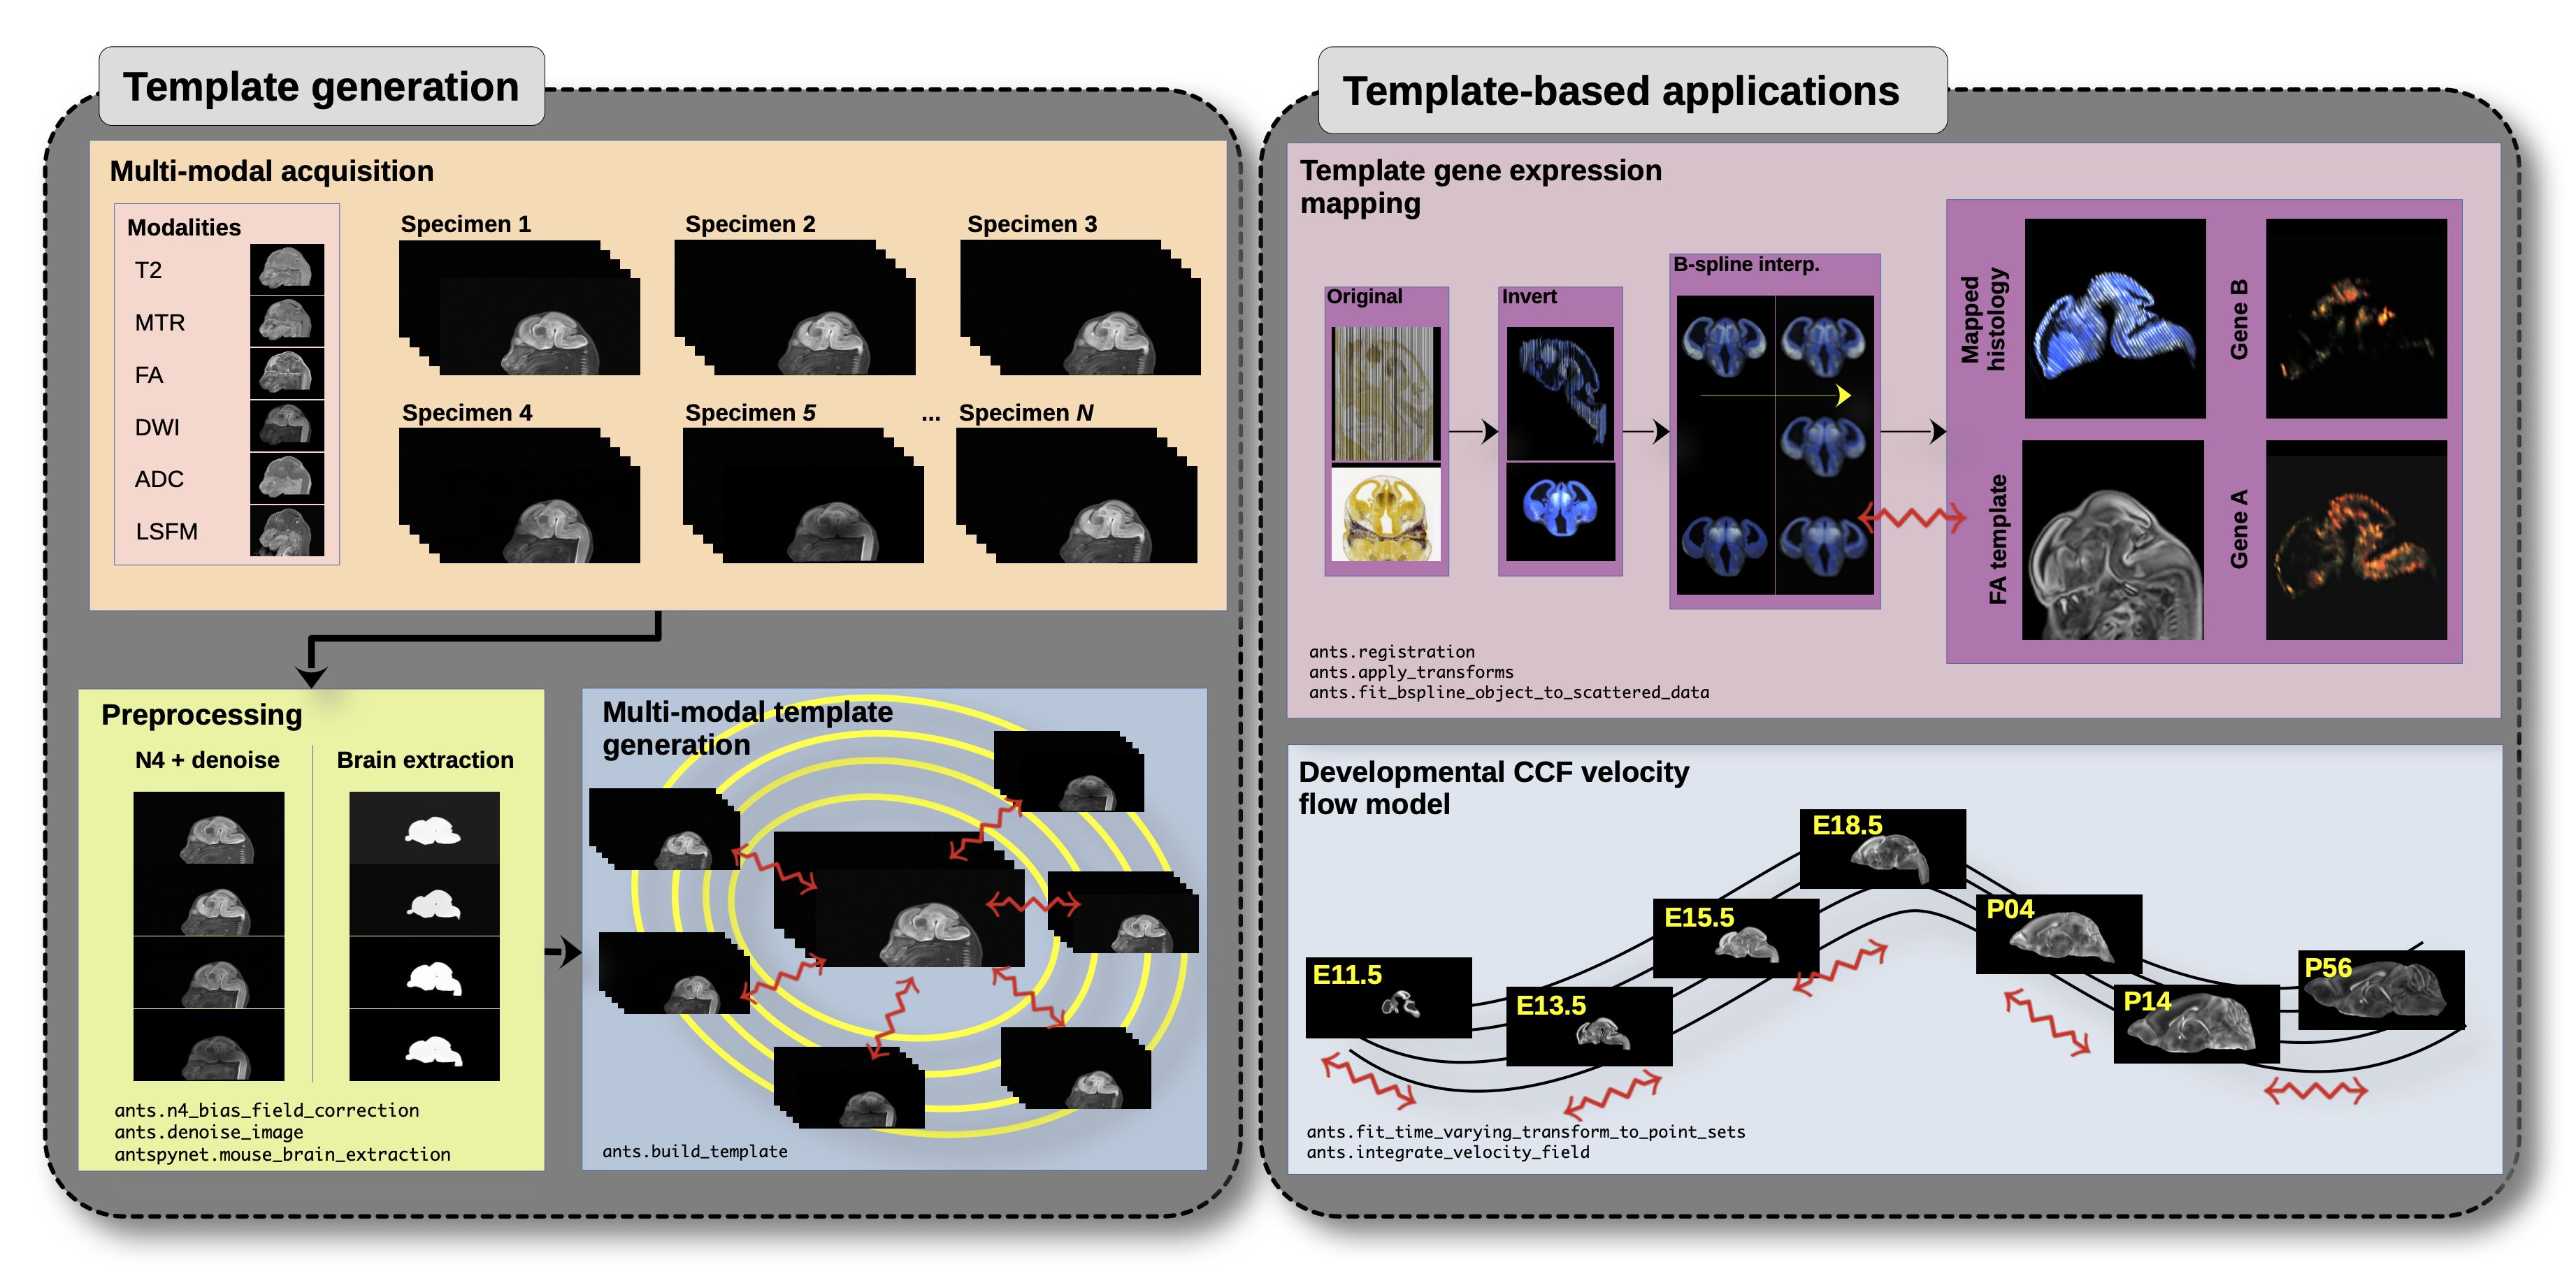
\includegraphics[width=1.2\textwidth]{Figures/pipeline3.png}}%
\caption{Illustration of a mouse brain template generation workflow and 
related template-based applications demonstrating the utility of different ANTsX
tools.  After imaging acquisition of the study population, various preprocessing
steps are applied to the imaging data such as bias correction, denoising, and
brain extraction as dictated by the needs of the study protocol.  In the specific 
case of the DevCCF, potential applications include gene expression mapping and the 
generation of the associated velocity flow model for continuous spatiotemporal 
mapping in the temporal domain spanned by the DevCCF.}
\label{fig:pipeline}
\end{figure}

Recently, the developmental common coordinate framework (DevCCF) was
introduced to the mouse brain research community as a public
resource.\textsuperscript{47} These symmetric atlases, comprising both
multimodal image data and anatomical segmentations defined by
developmental ontology, sample the mouse embryonic days (E) 11.5, E13.5,
E15.5, E18.5 and postnatal day (P) 4, P14, and P56. Modalities include
light sheet flourescence miscroscopy (LSFM) and at least four MRI
contrasts per developmental stage. Anatomical parcellations are also
available for each time point and were generated from ANTsX-based
mappings of gene expression and other cell type data. The P56 template
was integrated with the Allen CCFv3 to further increase the practical
utility of the DevCCF. These processes, specifically template generation
and multi-modal image mapping, were performed using ANTsX functionality
in the presence of previously noted image mapping difficulties (e.g.,
missing slices, tissue distortion).

Given the temporal gaps in the discrete set of developmental atlases
with the potential for additional interpolative time points, we discuss
the strategy of the current DevCCF template
generation\textsuperscript{47} and provide additional information for
the interested reader. Related, we also provide an open-source
framework, through ANTsX, for inferring correspondence within the
temporally continuous domain sampled by the existing set of embryonic
and postnatal atlases of the DevCCF. Although alternative approaches are
possible for interpolating between time points, this recently developed
ANTsX functionality permits the generation of a diffeomorphic velocity
flow transformation model,\textsuperscript{48} influenced by previous
work.\textsuperscript{49} The resulting time-parameterized velocity
field spans the stages of the DevCCF where mappings between any two
continuous time points within the span bounded by the E11.5 and P56
atlases is determined by integration of the optimized velocity field.
This functionality is available through ANTsX (via R and Python ANTsX
packages) with a dedicated GitHub repository that contains all data,
scripts, and other guidance necessary to both reproduce what is
described below and to illustrate how future researchers can incorporate
additional atlases into a more densely sampled model in a
straightforward manner.

\clearpage
\newpage

\hypertarget{results}{%
\section*{Results}\label{results}}
\addcontentsline{toc}{section}{Results}

\hypertarget{template-building}{%
\subsection*{Template building}\label{template-building}}
\addcontentsline{toc}{subsection}{Template building}

Template building using ANTsX tools was first described in the context
of hippocampal studies.\textsuperscript{50} Multi-modal and symmetrical
variants were subsequently described as part of a proposed brain tumor
segmentation approach based on random forests.\textsuperscript{51}
Template building capabilities are available in both ANTsPy
(\texttt{ants.build\_template(...)}) and ANTsR
(\texttt{buildTemplate(...)}) as well as part of the core ANTs package
(e.g., \texttt{antsMultivariateTemplateConstruction.sh}).

\hypertarget{data-preparation}{%
\subsubsection*{Data preparation}\label{data-preparation}}
\addcontentsline{toc}{subsubsection}{Data preparation}

Multi-modal symmetric template construction is performed separately for
each developmental stage. Prior to optimization, preprocessing can
include several steps not all of which are required but are dependent on
the data and the particular requirements of the study. For MRI scans,
inhomogeneity correction is often necessary and can be performed using
the ANTsPy function \texttt{ants.n4\_bias\_field\_correction(...)} which
is a wrapper for the N4 algorithm.\textsuperscript{24} Denoising is
another preprocessing step that can potentially improve template quality
results. The ANTsPy function \texttt{ants.denoise\_image(...)} is an
implementation of a well-known denoising algorithm.\textsuperscript{52}
For a typical image, both of these steps takes approximately on the
order of a couple minutes. In ANTsX, due to legacy code issues, only
bias correction is wrapped with template building so one need not
perform this step prior to optimization. In addition, brain extraction
has demonstrated improved performance in the context of human brain
normalization\textsuperscript{53} and is similarly used in mouse brain
registration to maximize alignment. Various approaches within ANTs are
possible including a template-based approach
\texttt{antsBrainExtraction.sh} or using deep learning
\texttt{antspynet.mouse\_brain\_extraction(...)}. Additionally, it is
important to ensure a standardized orientation, similar to the Dicom
standard for human brain imaging. A study requirement of template
bilateral symmetry is also an important consideration prior to template
generation. This can be performed by either flipping all the input
images contralaterally such that all input specimens are represented
twice or one can generate an initial asymmetric template, flipping it
contralaterally, and using the two asymmetric templates in a subsequent
template generation call to create a single symmetric template. For
multi-modal templates, all the images for a single specimen need to be
mutually aligned in the same image space prior to optimization. After
selecting the target image space for a particular specimen (e.g.,
T2-weighted MRI), this can be performed with a rigid transform
registration call using \texttt{ants.registration(...)}. It should be
noted that for most applications, the general hueristic of
\(\approx 10\) randomly sampled specimens is sufficient for a
satisfactory template.

In the case of the DevCCF, bias correction was employed in generating
the multiple stage templates using the shell script
\texttt{antsMultivariateConstruction.sh}. Brain extraction was applied
to the postnatal images. Template symmetrization employed the original
and contralateral versions of all specimen images.

\hypertarget{optimization}{%
\subsubsection*{Optimization}\label{optimization}}
\addcontentsline{toc}{subsubsection}{Optimization}

Template generation is initialized with either a user-provided image or
a bootstrapped initialization template constructed from the input data.
If the latter is selected, the voxelwise averaged image for each
modality is constructed followed by a linear registration of each
specimen to this template initialization which refines the estimate. The
former option is often used where computational considerations are
important. For example, this initial template can be generated using low
resolution input data or only a subset of the input cohort. This higher
quality initial estimate can then be further refined using the entire
data set at full resolution.

Following template initialization, each specimen is registered to the
current template estimate, which can be performed in parallel. After the
current round of registrations is complete, a voxelwise average of each
modality is performed with optional Laplacian sharpening followed by a
``shape update'' step. This shape update step is used to warp the
current estimate of the template so that its shape is closer to the mean
shape of the input data. Implementation-wise this is done by averaging
each displacement field that points from the template to the affinely
warped specimen. This average displacement field is then used to deform
the voxelwise-averaged template. Shape and intensity template
convergence typically occurs in four deformable iterations.

\hypertarget{the-devccf-velocity-flow-model}{%
\subsection*{The DevCCF Velocity Flow
Model}\label{the-devccf-velocity-flow-model}}
\addcontentsline{toc}{subsection}{The DevCCF Velocity Flow Model}

To continuously interpolate transformations between the different stages
of the DevCCF atlases, a velocity flow model was constructed using
Dev-CCF derived data and ANTsX functionality recently introduced into
both the ANTsR and ANTsPy packages. Both platforms include a complete
suite of functions for determining dense correspondence from sparse
landmarks based on a variety of transformation models ranging from
standard linear models (i.e., rigid, affine) to deformable diffeomorphic
models (e.g, symmetric normalization).\textsuperscript{39} The latter
set includes velocity flow models for both the pairwise scenario
(\texttt{ants.fit\_transform\_to\_paired\_points(...)}) and for multiple
sets
(\texttt{ants.fit\_time\_varying\_transform\_to\_point\_sets(...)}), as
in the case of the DevCCF. Several self-contained tutorials illustrating
usage for these functions are available at
\url{https://tinyurl.com/antsxtutorial}.

ANTsX, being built on top of ITK, uses an ITK image data structure for
the 4-D velocity field where each voxel contains the \(x\), \(y\), \(z\)
components of the field at that point. Field regularization is provided
by a B-spline scattered data approximation technique\textsuperscript{49}
which permits individual point weighting. Both field regularization and
integration of the velocity field are built on ITK functions contributed
from ANTsX development.

\hypertarget{data-preparation-1}{%
\subsubsection*{Data preparation}\label{data-preparation-1}}
\addcontentsline{toc}{subsubsection}{Data preparation}

\begin{figure}[!htb]
\centering
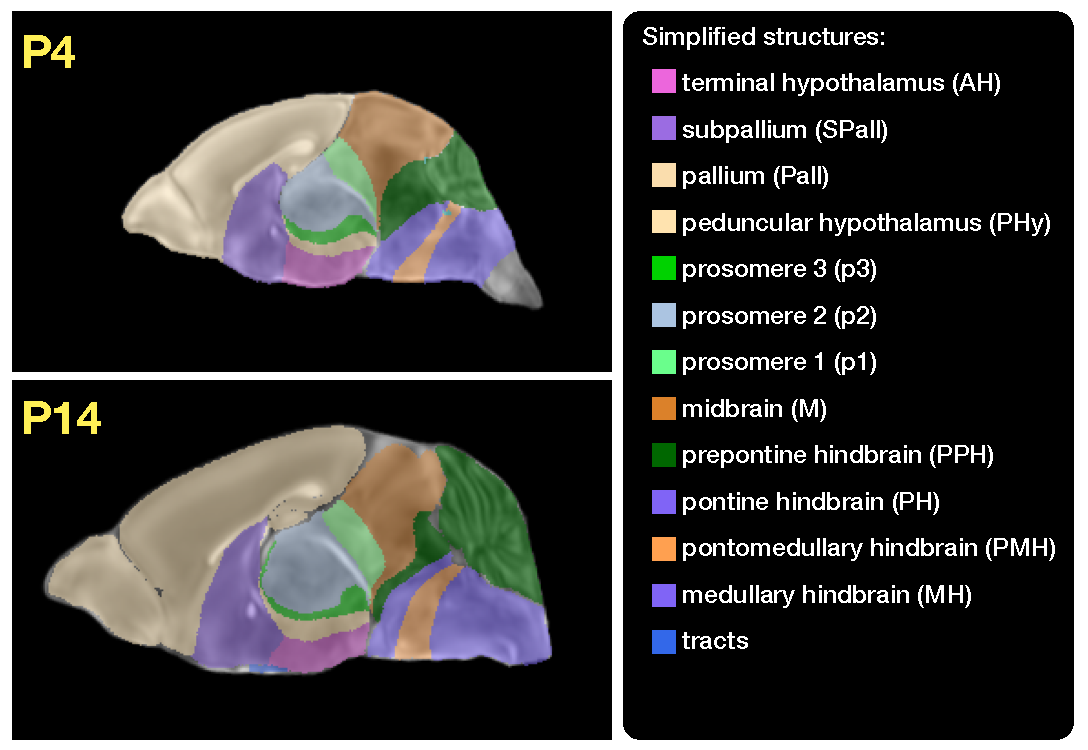
\includegraphics[width=0.75\textwidth]{Figures/SimplifiedAnnotations.pdf}
\caption{Annotated regions representing common labels across developmental stages which
are illustrated for both P4 and P14.}
\label{fig:simplifiedannotations}
\end{figure}

Labeled annotations are available as part of the original DevCCF and
reside in the space of each developmental template which range in
resolution from \(31.5-50 \mu\)m. Across all atlases, the total number
of labeled regions exceeds 2500. From these labels, a common set of 26
labels (13 per hemisphere) across all atlases were used for optimization
and evaluation. These regions are illustrated for the P4 and P14 stages
in Figure \ref{fig:simplifiedannotations}.

Prior to velocity field optimization, all data were rigidly transformed
to a common space. Using the centroids for the common label set of each
DevCCF atlas, each atlas was rigidly aligned to the space of the P56
atlas In order to determine the landmark correspondence across DevCCF
stages, the multi-metric capabilities of \texttt{ants.registration(...)}
were used. Instead of performing intensity-based pairwise registration
directly on these multi-label images, each label was used to construct a
separate fixed and moving image pair resulting in a multi-metric
registration optimization scenario involving 24 binary image pairs (each
label weighted equally) for optimizing diffeomorphic correspondence
between neighboring time point atlases using the mean squares metric and
the symmetric normalization transform.

To generate the set of common point sets across all seven developmental
atlases, the label boundaries and whole regions were sampled in the P56
atlas and then propagated to each atlas using the transformations
derived from the pairwise registrations. We selected a sampling rate of
10\% for the contour points and 1\% for the regional points for a total
number of points being per atlas being \(173303\)
(\(N_{contour} = 98151\) and \(N_{region}=75152\)). Regional boundary
points were weighted twice as those of regional points during
optimization.

\hypertarget{optimization-1}{%
\subsubsection*{Optimization}\label{optimization-1}}
\addcontentsline{toc}{subsubsection}{Optimization}

\begin{figure}[!htb]
\centering
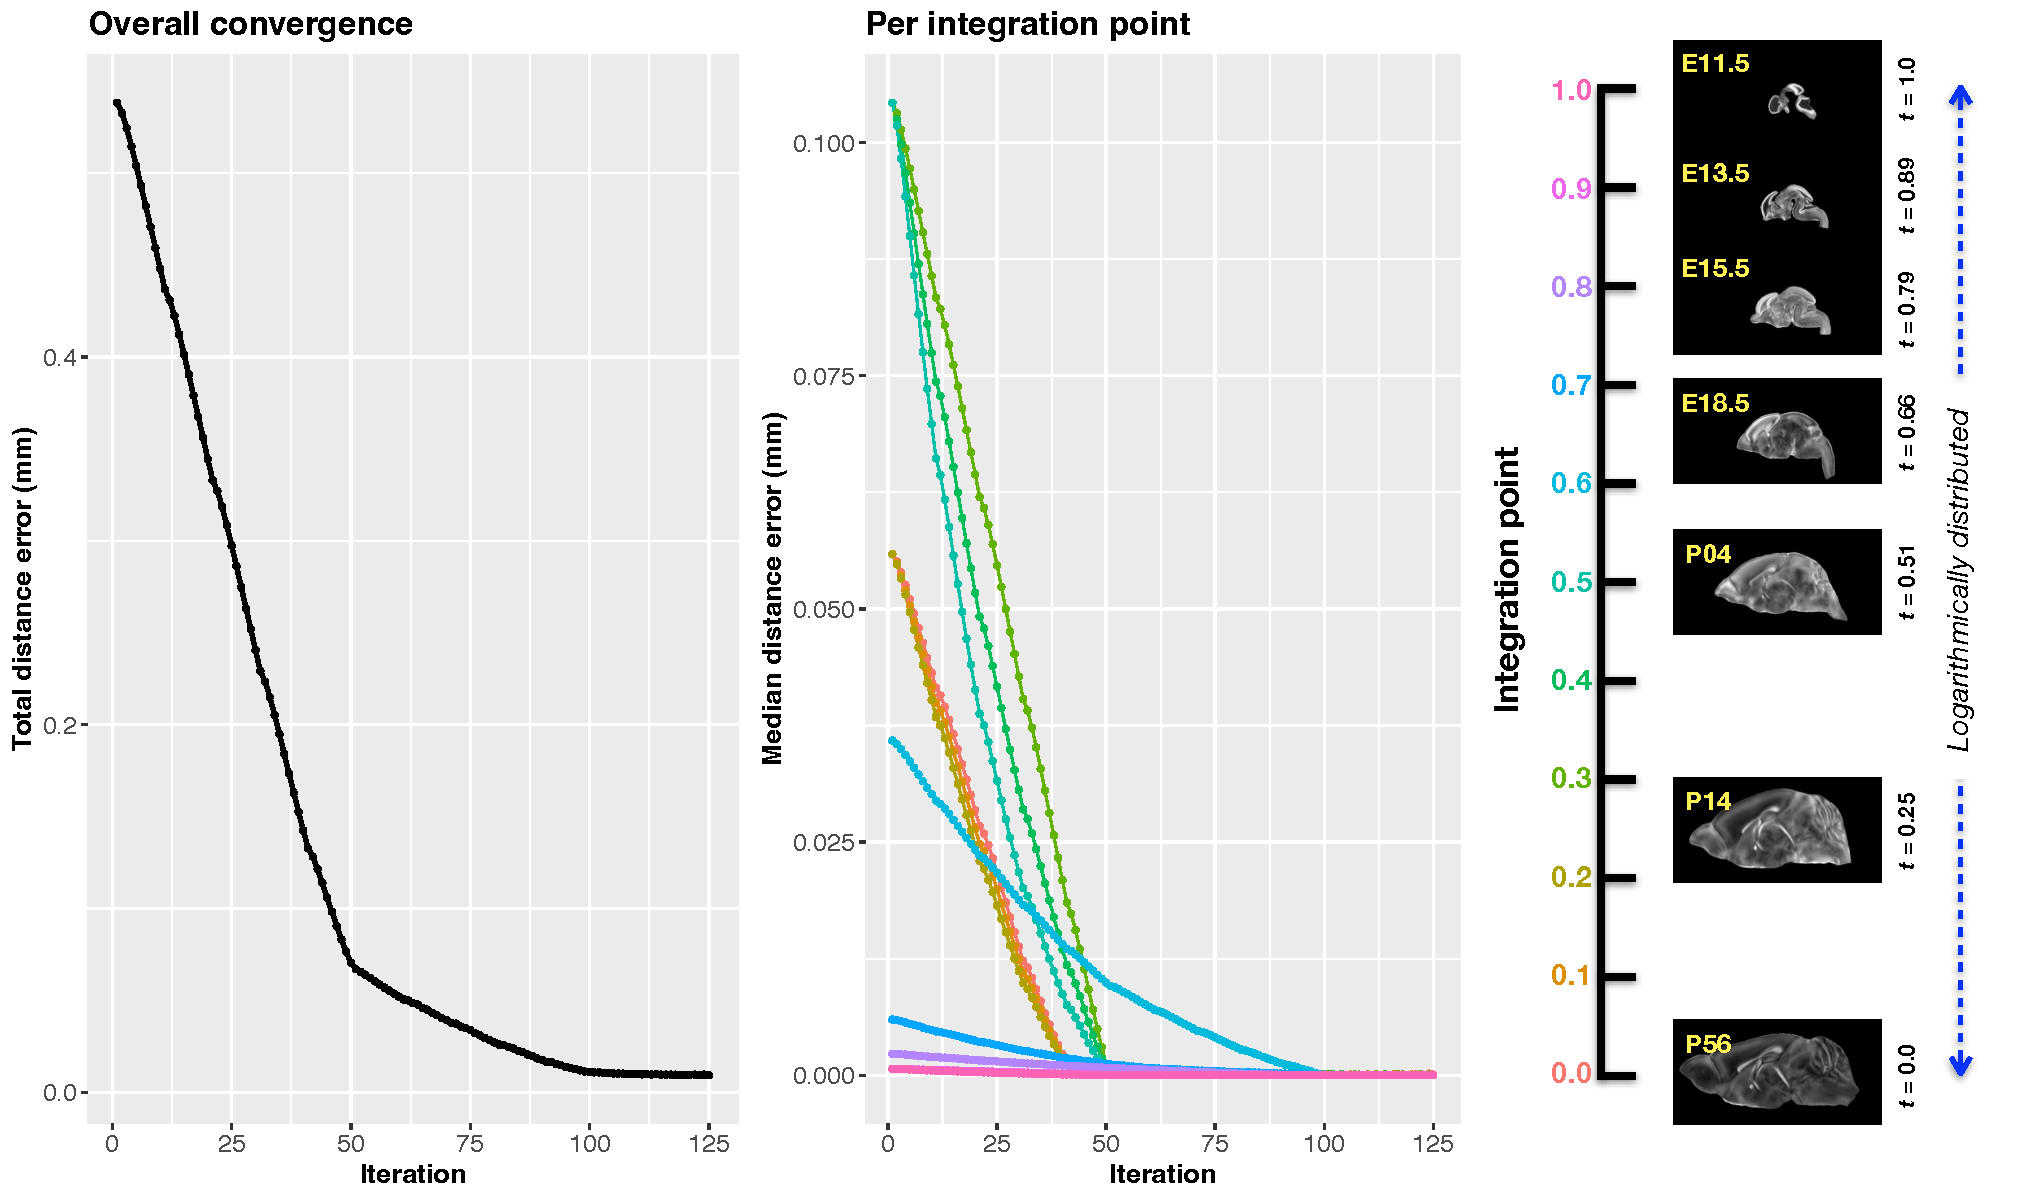
\includegraphics[width=0.99\textwidth]{Figures/convergence.pdf}
\caption{Convergence of the optimization of the velocity field for describing the 
transformation through the developmental stages from E11.5 through P56.}
\label{fig:convergence}
\end{figure}

\texttt{ants.fit\_time\_varying\_transform\_to\_point\_sets(...)} from
the ANTsPy package was used to optimize the velocity field. Input
comprised the seven corresponding point sets and their associated weight
values, the selected number of integration points for the velocity field
(\(N=11\)), and the parameters defining the geometry of the spatial
dimensions of the velocity field. Thus, the optimized velocity field
described here is of size \([256, 182, 360]\) (\(50 \mu\)m isotropic)
\(\times 11\) integration points for a total compressed size of a little
over 2 GB. This choice represented weighing the trade-off between
tractability, portability, and accuracy. However, all data and code to
reproduce the results described are available in a dedicated GitHub
repository (\url{https://github.com/ntustison/DevCCF-Velocity-Flow}).

The normalized time point scalar value for each atlas/point-set in the
temporal domains \([0, 1]\) was also defined. Given the increasingly
larger gaps in the postnatal timepoint sampling, we made two
adjustments. Based on known mouse brain development, we used 28 days for
the P56 data. We then computed the log transform of the adjusted set of
time points prior to normalization between 0 and 1 (see the right side
of Figure \ref{fig:convergence}). This log transform, as part of the
temporal normalization, significantly improved data spacing.

The max number of iterations was set to 200. At each iteration we looped
over the 11 integration points. At each integration point, the velocity
field estimate was updated by warping the two immediately adjacent point
sets to the integration time point and determining the regularized
displacement field between the two warped point sets. As with any
gradient-based descent algorithm, this field was multiplied by a small
step size (\(\delta = 0.2\)) before adding to the current velocity
field. Using multithreading, each iteration took about six minutes.

\begin{figure}[!htb]
\centering
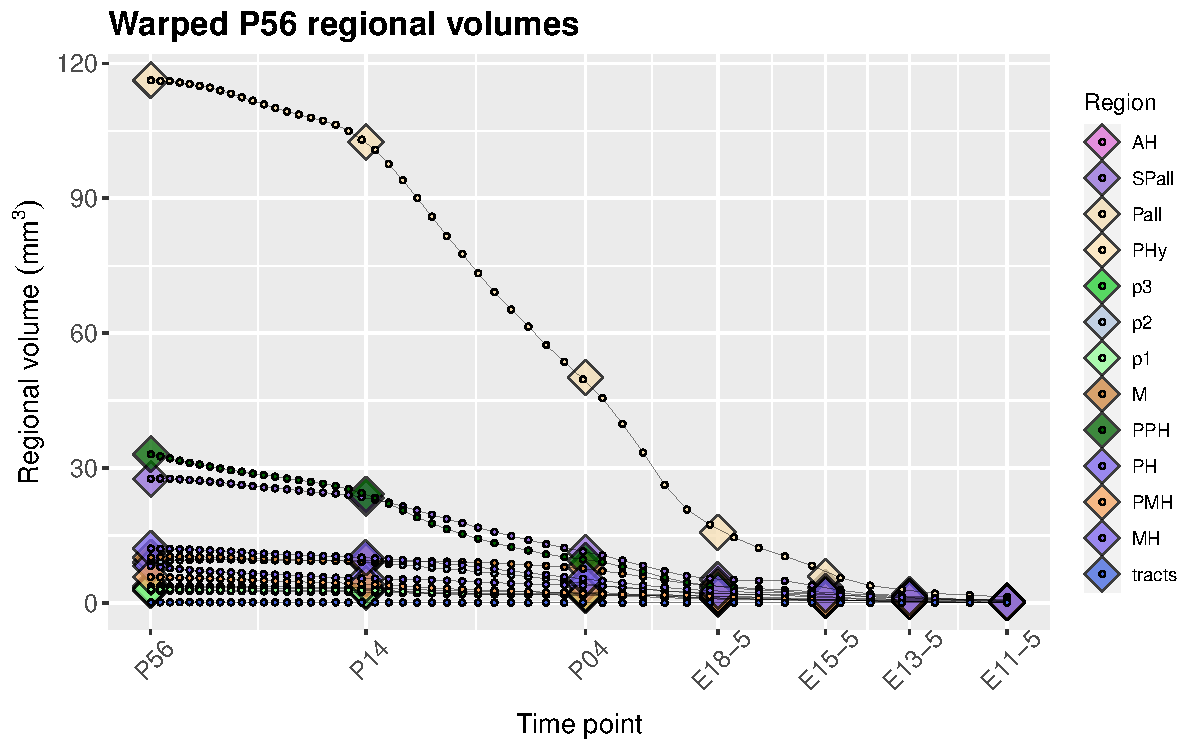
\includegraphics[width=0.75\textwidth]{Figures/warpedP56Volumes.pdf}
\caption{After the velocity field is generated, we can use it to warp
the simplified labels of the P56 atlas continuously over the interval
$[0, 1]$ and plot the volumes of the atlas regions.  Note how they 
compare with the volumes of the same regions in the other atlases.}
\label{fig:warpedP56}
\end{figure}

Convergence is determined by the average displacement error over each of
the integration points. As can be seen in the left panel of Figure
\ref{fig:convergence}, convergence occurred around 125 iterations when
the average displacement error over all integration points is minimized.
The median displacement error at each of the integration points also
trends towards zero but at different rates. After optimization, we use
the velocity field to warp the P56 set of labels to each of the other
atlas time points to compare the volumes of the different simplified
annotated regions. This is shown in Figure \ref{fig:warpedP56}.

\hypertarget{the-devccf-transform-model}{%
\subsubsection*{The DevCCF transform
model}\label{the-devccf-transform-model}}
\addcontentsline{toc}{subsubsection}{The DevCCF transform model}

\begin{figure}[!htb]
\centering
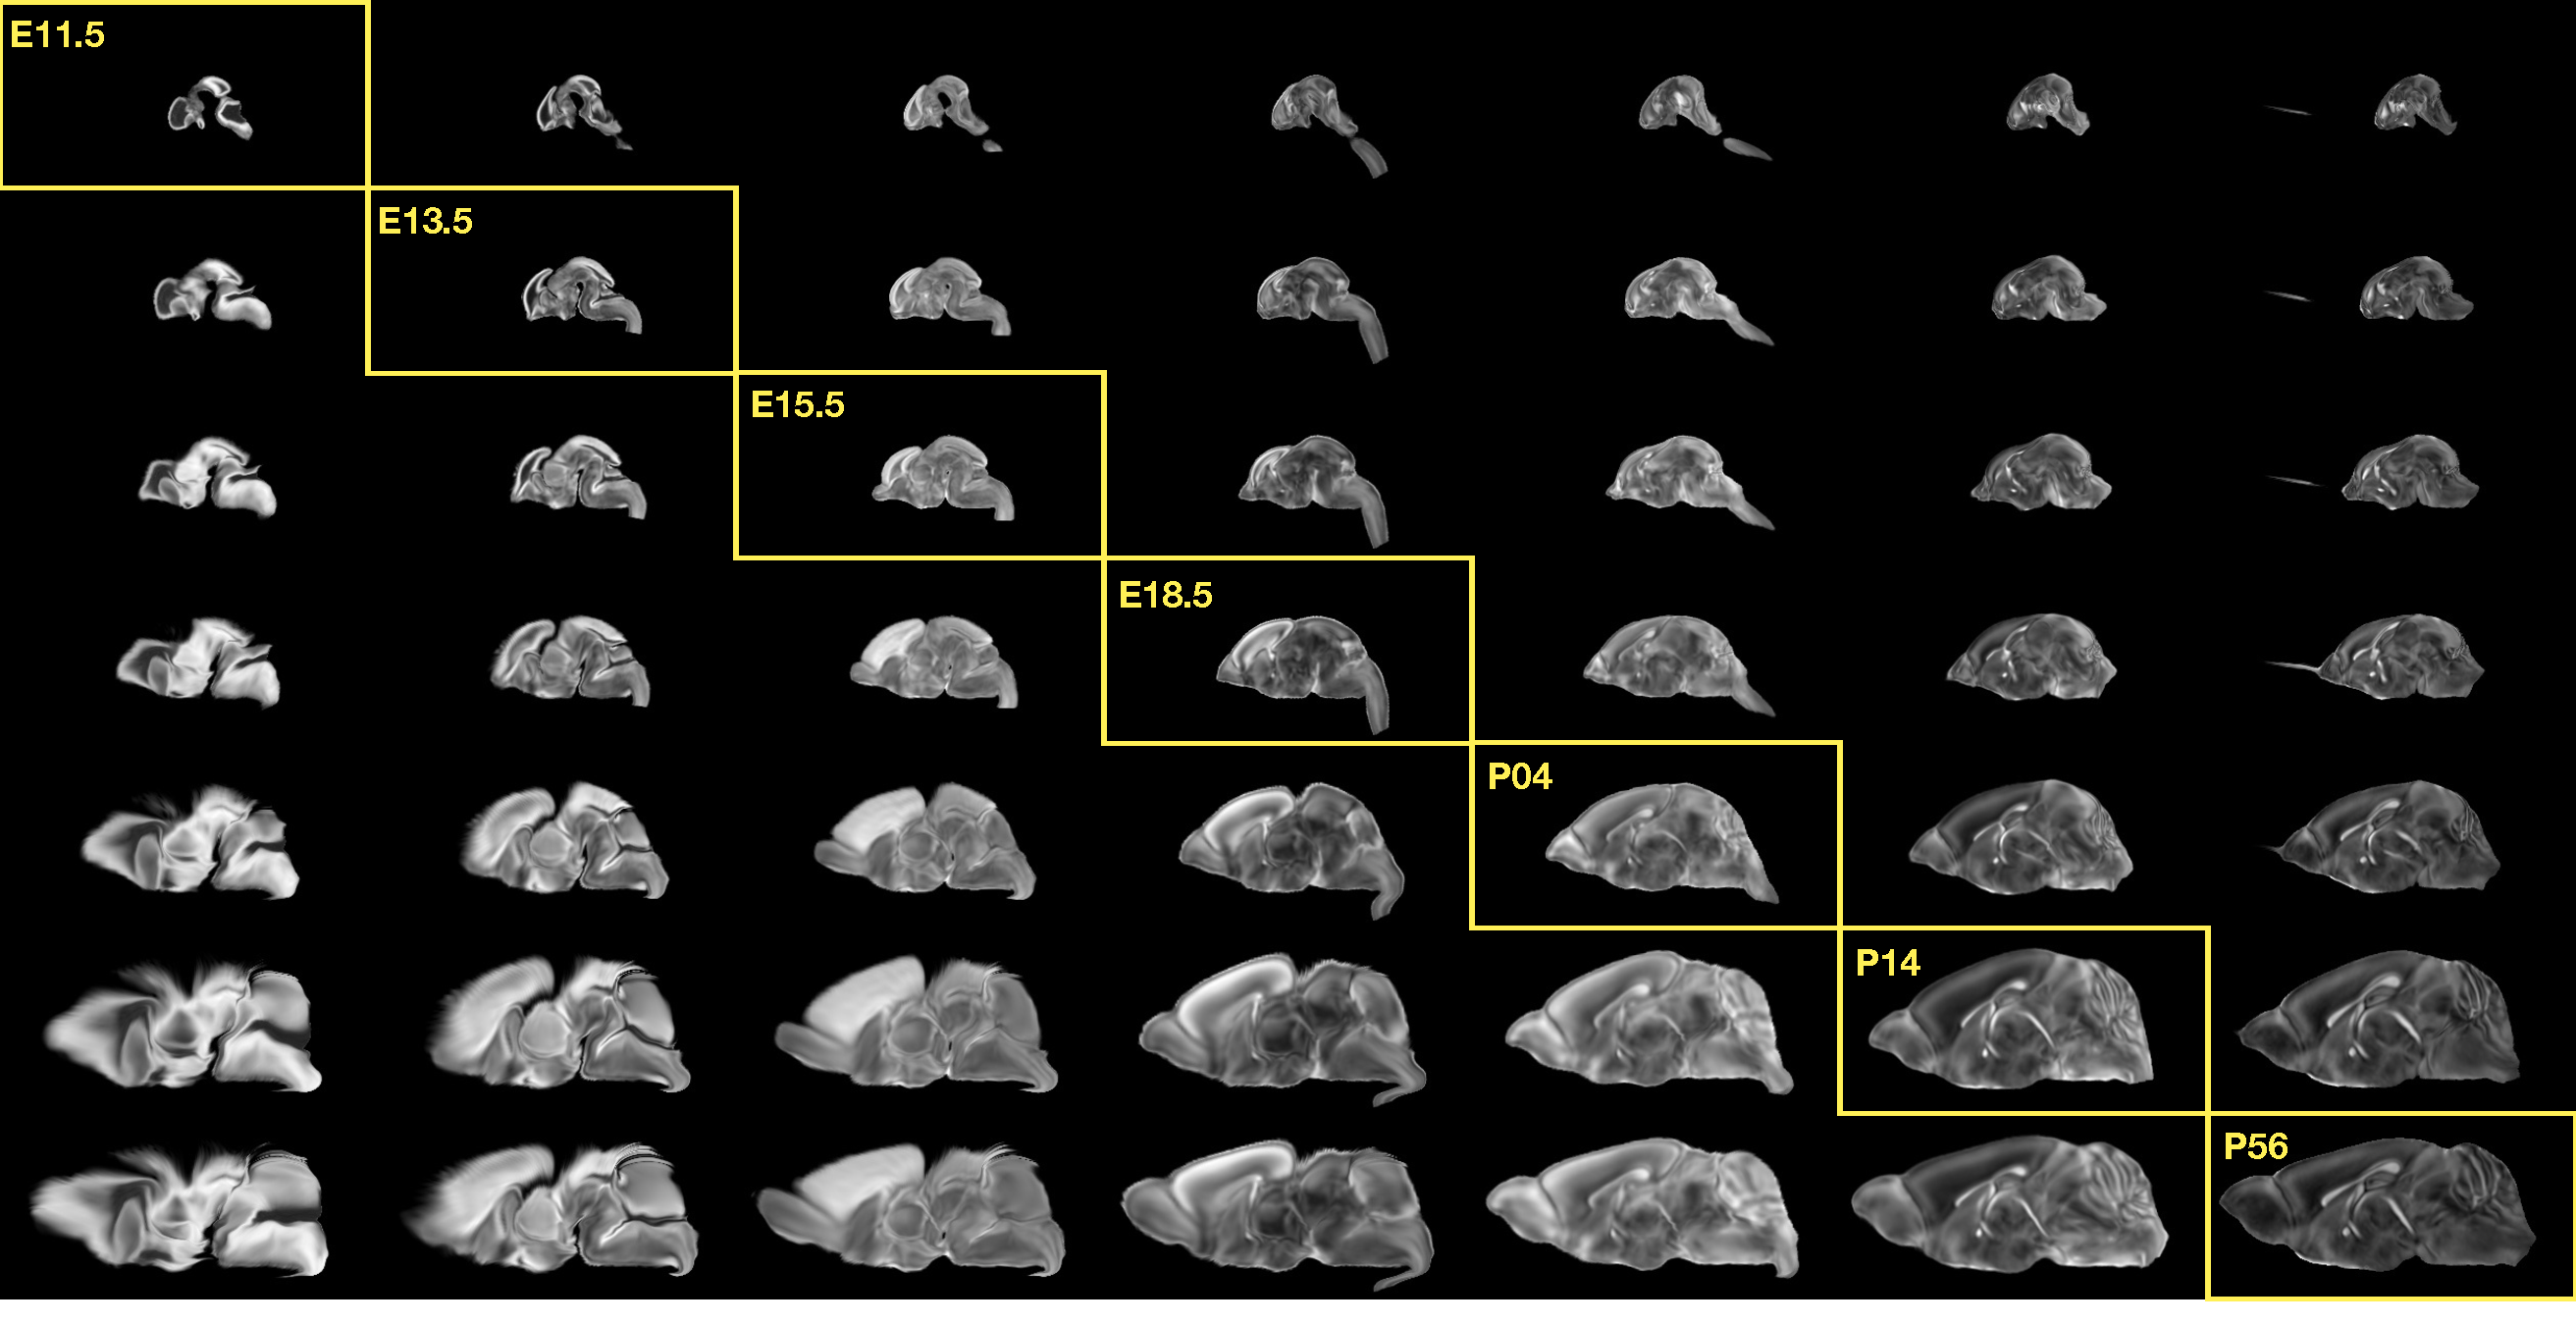
\includegraphics[width=0.99\textwidth]{Figures/CrossWarp.pdf}
\caption{Mid-sagittal visualization of the effects of the transformation model in
warping every developmental stage to the time point of every other developmental
stage.  The original images are located along the diagonal.  Columns correspond
to the warped original image whereas the rows represent the reference space to which
each image is warped.}
\label{fig:crosswarp}
\end{figure}

Once optimized, the resulting velocity field can be used to generate the
deformable transform between any two continuous points within the time
interval bounded by E11.5 and P56. In Figure \ref{fig:crosswarp}, we
transform each atlas to the space of every other atlas using the DevCCF
transform model. Additionally, one can use this transformation model to
construct virtual templates in the temporal gaps of the DevCCF. This is
illustrated in Figure \ref{fig:virtual} where we used the optimized
velocity field to construct virtual-templates at time point P10.3 and
P20---arbitrarily chosen simply to demonstrate the concept. After
situating these time points within the normalized time point interval,
the existing adjacent DevCCF atlases on either chronological side can be
warped to the desired time point. A subsequent call to one of the ANTsX
template building functions then permits the construction of the
template at that time point. Note that both of these usage examples can
be found on the GitHub repository given above.

\begin{figure}[!htb]
\centering
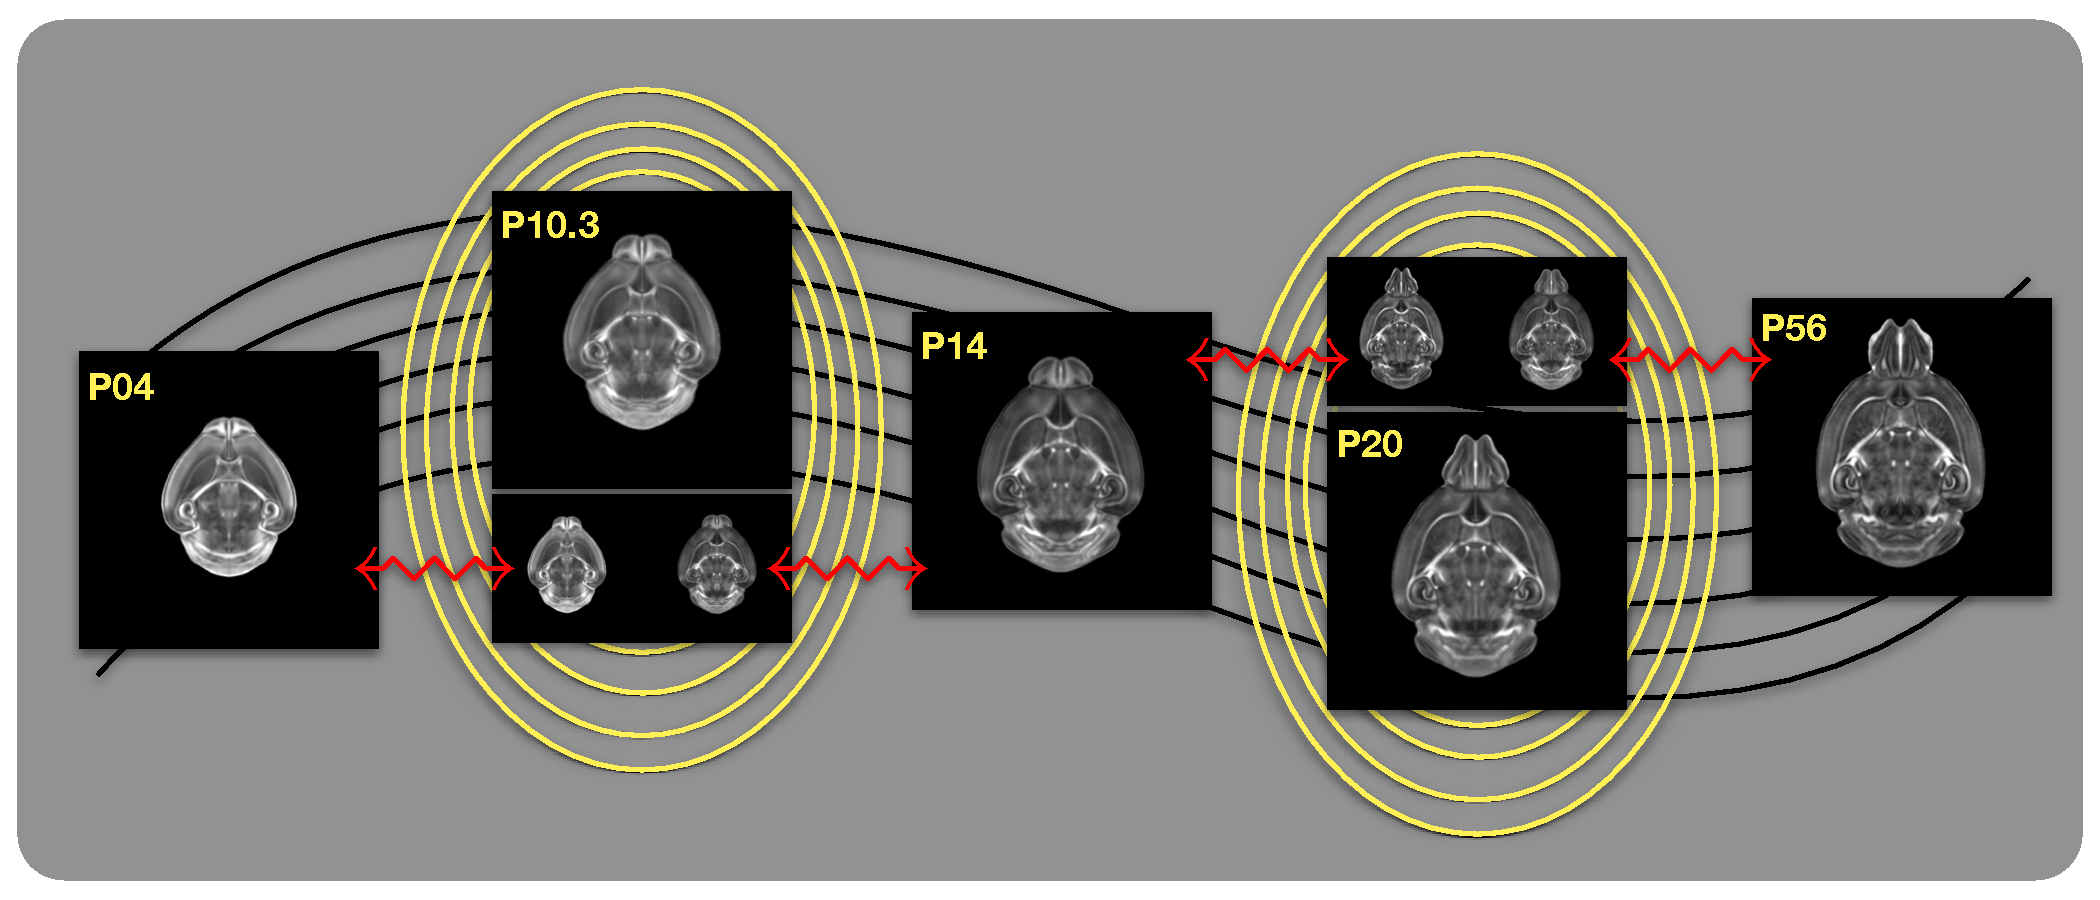
\includegraphics[width=0.99\textwidth]{Figures/pseudo_template.pdf}
\caption{Illustration of the use of the velocity flow model for creating virtual templates
at continuous time points not represented in one of the existing DevCCF time points.
For example, FA templates at time point P10.3 and P20 can be generated by warping the 
existing temporally adjacent developmental templates to the target time point and using 
those images in the ANTsX template building process.}
\label{fig:virtual}
\end{figure}

\clearpage
\newpage

\hypertarget{discussion}{%
\section*{Discussion}\label{discussion}}
\addcontentsline{toc}{section}{Discussion}

The ANTsX ecosystem is a powerful framework that has demonstrated
applicability to multiple species and organ systems, including the mouse
brain. This is further evidenced by the many other software packages
that use various ANTsX components in their own mouse-specific workflows.
The extensive functionality of ANTsX per se makes it possible to create
complete processing pipelines without requiring the integration of
multiple packages. These open-source ANTsX components not only perform
well but are available across multiple popular platforms which
facilitates the construction of tailored pipelines for individual study
solutions. These components are also supported by years of development
not only by the ANTsX development team but by the larger ITK community.

In the case of the development of the DevCCF, ANTsX was crucial in
providing necessary functionality for yielding high quality output.
First, for the generation of the individual developmental stage
multi-modal, symmetric templates, ANTsX is unique amongst image analysis
software packages in providing existing solutions for template
generation which have been thoroughly vetted, including being used in
several studies over the years, and which continue to be under active
refinement. At its core, computationally efficient and quality template
generation requires the use of precision pairwise image mapping
functionality which, historically, is at the origins of the ANTsX
ecosystem. And these mapping capabilities extend beyond template
generation to the mapping of other image data (e.g., gene expression
maps) to template for providing further insight into the mouse brain.

Despite the significant expansion of available developmental age
templates beyond what previously existed (e.g., Allen CCFv3), there
still exist temporal gaps in the DevCCF. However, pioneering work
involving diffeomorphic transformations allowed us to continuously
situate the existing templates within a time-varying velocity flow
model. This allows one to determine the diffeomorphic transformation
from any one temporal location to any other temporal location within the
time span defined by the E11.5 and P56 templates. This functionality is
built on multiple components from the Insight Segmentation and
Registraiton Toolkit including the B-spline scattered data approximation
technique for field regularization and velocity field integration using
fourth order Runge-Kutta. This velocity field model permits
intra-template comparison and the construction of virtual templates
where a template can be estimated at any continuous time point within
the temporal domain. This novel application can potentially enhance our
understanding of intermediate developmental stages. To increase its
impact and reproduce the results shown previously, we have made the data
and code publicly available at
\url{https://github.com/ntustison/DevCCF-Velocity-Flow}.

Although ANTsX is quite evolved in its development and functionality,
there are several areas which are currently under active development or
consideration for further expansion. Most notably, as in our human
applications, deep learning has had a significant impact in steering our
attention. Core functionality, such as brain extraction for mouse brain
mapping, would benefit from increasing the number of available
modalities. Additionally, as with much deep learning development, such
work will require additional data but is significantly facilitated by
the tools that we have created in both ANTsPyNet and ANTsRNet.

\clearpage
\newpage

\hypertarget{methods}{%
\section*{Methods}\label{methods}}
\addcontentsline{toc}{section}{Methods}

The following methods are all available as part of the ANTsX ecosystem
with analogous elements existing in both ANTsR (ANTs in R) and ANTsPy
(ANTs in Python) with and ANTs/ITK C++ core. However, most of the
development for the work described below was performed using ANTsPy. For
equivalent calls in ANTsR, please see the ANTsX tutorial at
\url{https://tinyurl.com/antsxtutorial}.

\hypertarget{preprocessing-bias-field-correction-and-denoising}{%
\subsection*{Preprocessing: bias field correction and
denoising}\label{preprocessing-bias-field-correction-and-denoising}}
\addcontentsline{toc}{subsection}{Preprocessing: bias field correction
and denoising}

As in human studies, bias field correction and image denoising are
standard preprocessing steps in improving overall image quality in mouse
brain images. The bias field, a gradual spatial intensity variation in
images, can arise from various sources such as magnetic field
inhomogeneity or acquisition artifacts, leading to distortions that can
compromise the quality of brain images. Correcting for bias fields
ensures a more uniform and consistent representation of brain
structures, enabling accurate quantitative analysis. Additionally, brain
images are often susceptible to various forms of noise, which can
obscure subtle features and affect the precision of measurements.
Denoising techniques help mitigate the impact of noise, enhancing the
signal-to-noise ratio and improving the overall image quality. The
well-known N4 bias field correction algorithm\textsuperscript{24} has
its origins in the ANTs toolkit which was implemented and introduced
into the ITK toolkit. Similarly, ANTsX contains an implementation of a
well-performing patch-based denoising technique\textsuperscript{52} and
is also available as an image filter to the ITK community.

\hypertarget{antsxnet-mouse-brain-applications}{%
\subsection*{ANTsXNet mouse brain
applications}\label{antsxnet-mouse-brain-applications}}
\addcontentsline{toc}{subsection}{ANTsXNet mouse brain applications}

\emph{General notes regarding deep learning training.}

All network-based approaches described below were implemented and
organized in the ANTsXNet libraries comprising Python (ANTsPyNet) and R
(ANTsRNet) analogs using the Keras/Tensorflow libraries available as
open-source in ANTsX GitHub repositories. For the various applications,
both share the identically trained weights for mutual reproducibility.
Training data was provided by manual labeling by various co-authors and
expanded using both intensity-based and shape-based data augmentation
techniques.

Intensity-based data augmentation consisted of randomly added noise
based on ITK functionality, simulated bias fields based on N4 bias field
modeling, and histogram warping for mimicking well-known MRI intensity
nonlinearities.\textsuperscript{25,55} These augmentation techniques are
available in ANTsXNet (only ANTsPyNet versions are listed): simulated
bias field: \texttt{antspynet.simulate\_bias\_field(...)}, image noise:
\texttt{antspyhet.add\_noise\_to\_image(...)}, and MRI intensity
nonlinear characterization:
\texttt{antspynet.histogram\_warp\_image\_intensities(...)}. Shape-based
data augmentation used both random linear and nonlinear deformations.
This functionality is also instantiated within ANTsXNet in terms of
random spatial warping:
\texttt{antspynet.randomly\_transform\_image\_data(...)}.

For all GPU training, we used Python scripts for creating custom batch
generators. As such batch generators tend to be application-specific, we
store them in a separate GitHub repository for public availability
(\url{https://github.com/ntustison/ANTsXNetTraining}). In terms of GPU
hardware, all training was done on a DGX (GPUs: 4X Tesla V100, system
memory: 256 GB LRDIMM DDR4).

\emph{Brain extraction.}

Similar to human neuroimage processing, brain extraction is a crucial
preprocessing step for accurate brain mapping. Within ANTsXNet, we have
created several deep learning networks for brain extraction for several
image modalities (e.g., T1, FLAIR, fractional anisotropy). Similarly,
for the developmental brain atlas work\textsuperscript{47} we developed
similar functionality for mouse brains of different modalities and
developmental age. All networks use a conventional 2-D U-net
architecture\textsuperscript{56} and perform prediction in a slice-wise
fashion given the limitations of the acquisition protocols (e.g.,
missing slices, slice thickness). Currently, coronal and sagittal
networks are available for both E13.5 and E15.5 data and coronal network
for T2-weighted MRI. In ANTsPyNet, this functionality is available in
the program \texttt{antspynet.mouse\_brain\_extraction(...)}. Even when
physical brain extraction is performed prior to image acquisition,
artifacts, such as bubbles or debris, can complicate subsequent
processing. Similar to the brain extraction networks, a 2-D U-net
architecture\textsuperscript{56} was created to separate the background
and foreground.

\emph{Miscellaneous networks: Super-resolution, cerebellum, and
hemispherical masking.}

To further enhance the data prior to designing mapping protocols,
additional networks were created. A well-performing deep back projection
network\textsuperscript{57} was ported to ANTsXNet and expanded to 3-D
for various super-resolution applications,\textsuperscript{58} including
mouse data. Finally, features of anatomical significance, namely the
cerebellum and hemispherical midline were captured in these data using
deep learning networks.

\hypertarget{intra-slice-image-registration-with-missing-slice-imputation}{%
\subsection*{Intra-slice image registration with missing slice
imputation}\label{intra-slice-image-registration-with-missing-slice-imputation}}
\addcontentsline{toc}{subsection}{Intra-slice image registration with
missing slice imputation}

Volumetric gene expression slice data was collated into 3-D volumes.
Prior to mapping this volume to the corresponding structural data and,
potentially, to the appropriate template, alignment was improved using
deformable registration on contiguous slices. However, one of the
complications associated with these image data was the unknown number of
missing slices, the number of consecutive missing slices, and the
different locations of these missing slices. To handle this missing data
problem, we found that data interpolation using the B-spline
approximation algorithm cited earlier\textsuperscript{54} (ANTsPy
function: \texttt{ants.fit\_bspline\_object\_to\_scattered\_data(...)}).
This provided sufficient data interpolation fidelity to perform
continuous slicewise registration. Other possible variants that were
considered but deemed unnecessary was performing more than one iteration
cycling through data interpolation and slicewise alignment. The other
possibility was incorporating the super-resolution technique described
earlier. But again, our data did not require these additional steps.

\hypertarget{image-registration}{%
\subsection*{Image registration}\label{image-registration}}
\addcontentsline{toc}{subsection}{Image registration}

The ANTs registration toolkit is a complex framework permitting highly
tailored solutions to pairwise image registration
scenarios.\textsuperscript{59} It includes innovative transformation
models for biological modeling\textsuperscript{39,49} and has proven
capable of excellent performance.\textsuperscript{40,60} Various
parameter sets targeting specific applications have been packaged with
the different ANTsX platforms, specifically ANTs, ANTsPy, and
ANTsR.\textsuperscript{25} In ANTsPy, the function
\texttt{ants.registration(...)} is used to register a pair of images or
a pair of image sets where \texttt{type\_of\_transform} is a
user-specified option that invokes a specific parameter set. For example
\texttt{type\_of\_transform=\textquotesingle{}antsRegistrationSyNQuick{[}s{]}\textquotesingle{}}
is an oft-used parameter set.

Initially, linear optimization is initialized with center of (intensity)
mass alignment typically followed by optimization of both rigid and
affine transforms using the mutual information similarity metric. This
is followed by diffeomorphic deformable alignment using symmetric
normalization (SyN) with Gaussian\textsuperscript{39} or B-spline
regularization\textsuperscript{49} where the forward transform is
invertible and differentiable. The similarity metric employed at this
latter stage is typically either neighborhood cross-correlation or
mutual information. Note that these parameter sets are robust to input
image type (i.e., LSFM, Nissl staining, and the various MRI modalities)
and are adaptable to mousing image geometry scaling. Further details can
be found in the various documentation sources for these ANTsX packages.

\hypertarget{template-generation}{%
\subsection*{Template generation}\label{template-generation}}
\addcontentsline{toc}{subsection}{Template generation}

ANTsX provides functionality for constructing templates from a set (or
multi-modal sets) of input images as originally
described\textsuperscript{50} and recently used to create the DevCCF
templates.\textsuperscript{47} An initial template estimate is
constructed from an existing subject image or a voxelwise average
derived from a rigid pre-alignment of the image population. Pairwise
registration between each subject and the current template estimate is
performed using the Symmetric Normalization (SyN)
algorithm.\textsuperscript{39} The template estimate is updated by
warping all subjects to the space of the template, performing a
voxelwise average, and then performing a ``shape update'' of this latter
image by warping it by the average inverse deformation, thus yielding a
mean image of the population in terms of both intensity and shape.

\hypertarget{continuous-developmental-velocity-flow-transformation-model}{%
\subsection*{Continuous developmental velocity flow transformation
model}\label{continuous-developmental-velocity-flow-transformation-model}}
\addcontentsline{toc}{subsection}{Continuous developmental velocity flow
transformation model}

Given multiple, linearly or non-linearly ordered point sets where
individual points across are in one-to-one correspondence, we developed
an approach for generating a velocity flow transformation model to
describe a time-varying diffeomorphic mapping as a variant of the
inexact landmark matching solution. Integration of the resulting
velocity field can then be used to describe the displacement between any
two time points within this time-parameterized domain. Regularization of
the sparse correspondence between point sets is performed using a
generalized B-spline scattered data approximation
technique,\textsuperscript{54} also developed by the ANTsX developers
and contributed to ITK.

To apply this methodology to the developmental
templates,\textsuperscript{47} we coalesced the manual parcellations of
the developmental templates into 26 common anatomical regions (13 per
hemisphere). We then used these regions to generate invertible
transformations between successive time points. Specifically each label
was used to create a pair of single region images resulting in 26 pairs
of ``source'' and ``target'' images. The multiple image pairs were used
to iteratively estimate a diffeomorphic pairwise transform. Given the
seven atlases E11.5, E13.5, E15.5, E18.5, P4, P14, and P56, this
resulted in 6 sets of transforms between successive time points. Given
the relative sizes between atlases, on the order of 10\(^6\) points were
randomly sampled labelwise in the P56 template space and propagated to
each successive atlas providing the point sets for constructing the
velocity flow model. Approximately 125 iterations resulted in a steady
convergence based on the average Euclidean norm between transformed
point sets. Ten integration points were used and point sets were
distributed along the temporal dimension using a log transform for a
more evenly spaced sampling.

\hypertarget{visualization}{%
\subsection*{Visualization}\label{visualization}}
\addcontentsline{toc}{subsection}{Visualization}

To complement the well-known visualization capabilities of R and Python,
e.g., ggplot2 and matplotlib, respectively, image-specific visualization
capabilities are available in the \texttt{ants.plot(...)} (Python) and
\texttt{plot.antsImage(...)} (R). These are capable of illustrating
multiple slices in different orientations with both other image overlays
as well as label images.

\clearpage
\newpage

\textbf{Data availability.} All data used in this work are publicly
available. The DevCCF atlas is available at
\url{https://kimlab.io/brain-map/DevCCF/}. Additionally, all software
discussed is publicly available. ANTsPy and ANTsR are available through
GitHub at the ANTsX Ecosystem (\url{https://github.com/ANTsX}). A GitHub
repository specific to the work discussed in the manuscript was created
and is available at
\url{https://github.com/ntustison/DevCCF-Velocity-Flow}.

\clearpage

\hypertarget{references}{%
\section*{References}\label{references}}
\addcontentsline{toc}{section}{References}

\hypertarget{refs}{}
\begin{CSLReferences}{0}{0}
\leavevmode\vadjust pre{\hypertarget{ref-Keller:2015aa}{}}%
\CSLLeftMargin{1. }
\CSLRightInline{Keller, P. J. \& Ahrens, M. B. Visualizing whole-brain
activity and development at the single-cell level using light-sheet
microscopy. \emph{Neuron} \textbf{85}, 462--83 (2015).}

\leavevmode\vadjust pre{\hypertarget{ref-La-Manno:2021aa}{}}%
\CSLLeftMargin{2. }
\CSLRightInline{La Manno, G. \emph{et al.} Molecular architecture of the
developing mouse brain. \emph{Nature} \textbf{596}, 92--96 (2021).}

\leavevmode\vadjust pre{\hypertarget{ref-Wen:2022aa}{}}%
\CSLLeftMargin{3. }
\CSLRightInline{Wen, L. \emph{et al.} Single-cell technologies: From
research to application. \emph{Innovation (Camb)} \textbf{3}, 100342
(2022).}

\leavevmode\vadjust pre{\hypertarget{ref-Oh:2014aa}{}}%
\CSLLeftMargin{4. }
\CSLRightInline{Oh, S. W. \emph{et al.} A mesoscale connectome of the
mouse brain. \emph{Nature} \textbf{508}, 207--14 (2014).}

\leavevmode\vadjust pre{\hypertarget{ref-Gong:2013aa}{}}%
\CSLLeftMargin{5. }
\CSLRightInline{Gong, H. \emph{et al.} Continuously tracing brain-wide
long-distance axonal projections in mice at a one-micron voxel
resolution. \emph{Neuroimage} \textbf{74}, 87--98 (2013).}

\leavevmode\vadjust pre{\hypertarget{ref-Li:2010aa}{}}%
\CSLLeftMargin{6. }
\CSLRightInline{Li, A. \emph{et al.} Micro-optical sectioning tomography
to obtain a high-resolution atlas of the mouse brain. \emph{Science}
\textbf{330}, 1404--8 (2010).}

\leavevmode\vadjust pre{\hypertarget{ref-Ueda:2020aa}{}}%
\CSLLeftMargin{7. }
\CSLRightInline{Ueda, H. R. \emph{et al.} Tissue clearing and its
applications in neuroscience. \emph{Nat Rev Neurosci} \textbf{21},
61--79 (2020).}

\leavevmode\vadjust pre{\hypertarget{ref-Stahl:2016aa}{}}%
\CSLLeftMargin{8. }
\CSLRightInline{Ståhl, P. L. \emph{et al.} Visualization and analysis of
gene expression in tissue sections by spatial transcriptomics.
\emph{Science} \textbf{353}, 78--82 (2016).}

\leavevmode\vadjust pre{\hypertarget{ref-Burgess:2019aa}{}}%
\CSLLeftMargin{9. }
\CSLRightInline{Burgess, D. J. Spatial transcriptomics coming of age.
\emph{Nat Rev Genet} \textbf{20}, 317 (2019).}

\leavevmode\vadjust pre{\hypertarget{ref-MacKenzie-Graham:2004aa}{}}%
\CSLLeftMargin{10. }
\CSLRightInline{MacKenzie-Graham, A. \emph{et al.} A multimodal,
multidimensional atlas of the C57BL/6J mouse brain. \emph{J Anat}
\textbf{204}, 93--102 (2004).}

\leavevmode\vadjust pre{\hypertarget{ref-Mackenzie-Graham:2007aa}{}}%
\CSLLeftMargin{11. }
\CSLRightInline{Mackenzie-Graham, A. J. \emph{et al.} Multimodal,
multidimensional models of mouse brain. \emph{Epilepsia} \textbf{48
Suppl 4}, 75--81 (2007).}

\leavevmode\vadjust pre{\hypertarget{ref-Dong:2008aa}{}}%
\CSLLeftMargin{12. }
\CSLRightInline{Dong, H. W. \emph{Allen reference atlas. A digital color
brain atlas of the C57BL/6J male mouse}. (John Wiley; Sons, 2008).}

\leavevmode\vadjust pre{\hypertarget{ref-Wang:2020aa}{}}%
\CSLLeftMargin{13. }
\CSLRightInline{Wang, Q. \emph{et al.} The allen mouse brain common
coordinate framework: A 3D reference atlas. \emph{Cell} \textbf{181},
936--953.e20 (2020).}

\leavevmode\vadjust pre{\hypertarget{ref-Johnson:2010aa}{}}%
\CSLLeftMargin{14. }
\CSLRightInline{Johnson, G. A. \emph{et al.} Waxholm space: An
image-based reference for coordinating mouse brain research.
\emph{Neuroimage} \textbf{53}, 365--72 (2010).}

\leavevmode\vadjust pre{\hypertarget{ref-Oguz:2014aa}{}}%
\CSLLeftMargin{15. }
\CSLRightInline{Oguz, I., Zhang, H., Rumple, A. \& Sonka, M. RATS: Rapid
automatic tissue segmentation in rodent brain MRI. \emph{J Neurosci
Methods} \textbf{221}, 175--82 (2014).}

\leavevmode\vadjust pre{\hypertarget{ref-Sawiak:2014aa}{}}%
\CSLLeftMargin{16. }
\CSLRightInline{Sawiak, S. J., Picq, J.-L. \& Dhenain, M. Voxel-based
morphometry analyses of in vivo MRI in the aging mouse lemur primate.
\emph{Front Aging Neurosci} \textbf{6}, 82 (2014).}

\leavevmode\vadjust pre{\hypertarget{ref-Ashburner:2012aa}{}}%
\CSLLeftMargin{17. }
\CSLRightInline{Ashburner, J. {SPM}: A history. \emph{Neuroimage}
\textbf{62}, 791--800 (2012).}

\leavevmode\vadjust pre{\hypertarget{ref-Modat:2010aa}{}}%
\CSLLeftMargin{18. }
\CSLRightInline{Modat, M. \emph{et al.} Fast free-form deformation using
graphics processing units. \emph{Comput Methods Programs Biomed}
\textbf{98}, 278--84 (2010).}

\leavevmode\vadjust pre{\hypertarget{ref-Tyson:2022aa}{}}%
\CSLLeftMargin{19. }
\CSLRightInline{Tyson, A. L. \emph{et al.} Accurate determination of
marker location within whole-brain microscopy images. \emph{Sci Rep}
\textbf{12}, 867 (2022).}

\leavevmode\vadjust pre{\hypertarget{ref-Pallast:2019aa}{}}%
\CSLLeftMargin{20. }
\CSLRightInline{Pallast, N. \emph{et al.} Processing pipeline for
atlas-based imaging data analysis of structural and functional mouse
brain MRI (AIDAmri). \emph{Front Neuroinform} \textbf{13}, 42 (2019).}

\leavevmode\vadjust pre{\hypertarget{ref-Jenkinson:2012wi}{}}%
\CSLLeftMargin{21. }
\CSLRightInline{Jenkinson, M., Beckmann, C. F., Behrens, T. E. J.,
Woolrich, M. W. \& Smith, S. M. FSL. \emph{Neuroimage} \textbf{62},
782--90 (2012).}

\leavevmode\vadjust pre{\hypertarget{ref-Yeh:2010aa}{}}%
\CSLLeftMargin{22. }
\CSLRightInline{Yeh, F.-C., Wedeen, V. J. \& Tseng, W.-Y. I. Generalized
q-sampling imaging. \emph{IEEE Trans Med Imaging} \textbf{29}, 1626--35
(2010).}

\leavevmode\vadjust pre{\hypertarget{ref-Jorge-Cardoso:2013aa}{}}%
\CSLLeftMargin{23. }
\CSLRightInline{Jorge Cardoso, M. \emph{et al.} STEPS: Similarity and
truth estimation for propagated segmentations and its application to
hippocampal segmentation and brain parcelation. \emph{Med Image Anal}
\textbf{17}, 671--84 (2013).}

\leavevmode\vadjust pre{\hypertarget{ref-Tustison:2010ac}{}}%
\CSLLeftMargin{24. }
\CSLRightInline{Tustison, N. J. \emph{et al.} {N4ITK}: Improved {N3}
bias correction. \emph{IEEE Trans Med Imaging} \textbf{29}, 1310--20
(2010).}

\leavevmode\vadjust pre{\hypertarget{ref-Tustison:2021aa}{}}%
\CSLLeftMargin{25. }
\CSLRightInline{Tustison, N. J. \emph{et al.} The ANTsX ecosystem for
quantitative biological and medical imaging. \emph{Sci Rep} \textbf{11},
9068 (2021).}

\leavevmode\vadjust pre{\hypertarget{ref-Goubran:2019aa}{}}%
\CSLLeftMargin{26. }
\CSLRightInline{Goubran, M. \emph{et al.} Multimodal image registration
and connectivity analysis for integration of connectomic data from
microscopy to MRI. \emph{Nat Commun} \textbf{10}, 5504 (2019).}

\leavevmode\vadjust pre{\hypertarget{ref-Celestine:2020aa}{}}%
\CSLLeftMargin{27. }
\CSLRightInline{Celestine, M., Nadkarni, N. A., Garin, C. M., Bougacha,
S. \& Dhenain, M. Sammba-MRI: A library for processing SmAll-MaMmal
BrAin MRI data in python. \emph{Front Neuroinform} \textbf{14}, 24
(2020).}

\leavevmode\vadjust pre{\hypertarget{ref-Ioanas:2021aa}{}}%
\CSLLeftMargin{28. }
\CSLRightInline{Ioanas, H.-I., Marks, M., Zerbi, V., Yanik, M. F. \&
Rudin, M. An optimized registration workflow and standard geometric
space for small animal brain imaging. \emph{Neuroimage} \textbf{241},
118386 (2021).}

\leavevmode\vadjust pre{\hypertarget{ref-Cox:2012aa}{}}%
\CSLLeftMargin{29. }
\CSLRightInline{Cox, R. W. {AFNI}: What a long strange trip it's been.
\emph{Neuroimage} \textbf{62}, 743--7 (2012).}

\leavevmode\vadjust pre{\hypertarget{ref-Ni:2020aa}{}}%
\CSLLeftMargin{30. }
\CSLRightInline{Ni, H. \emph{et al.} A robust image registration
interface for large volume brain atlas. \emph{Sci Rep} \textbf{10}, 2139
(2020).}

\leavevmode\vadjust pre{\hypertarget{ref-Jin:2022aa}{}}%
\CSLLeftMargin{31. }
\CSLRightInline{Jin, M. \emph{et al.} SMART: An open-source extension of
WholeBrain for intact mouse brain registration and segmentation.
\emph{eNeuro} \textbf{9}, (2022).}

\leavevmode\vadjust pre{\hypertarget{ref-Furth:2018aa}{}}%
\CSLLeftMargin{32. }
\CSLRightInline{Fürth, D. \emph{et al.} An interactive framework for
whole-brain maps at cellular resolution. \emph{Nat Neurosci}
\textbf{21}, 139--149 (2018).}

\leavevmode\vadjust pre{\hypertarget{ref-Negwer:2022aa}{}}%
\CSLLeftMargin{33. }
\CSLRightInline{Negwer, M. \emph{et al.} FriendlyClearMap: An optimized
toolkit for mouse brain mapping and analysis. \emph{Gigascience}
\textbf{12}, (2022).}

\leavevmode\vadjust pre{\hypertarget{ref-Klein:2010aa}{}}%
\CSLLeftMargin{34. }
\CSLRightInline{Klein, S., Staring, M., Murphy, K., Viergever, M. A. \&
Pluim, J. P. W. Elastix: A toolbox for intensity-based medical image
registration. \emph{IEEE Trans Med Imaging} \textbf{29}, 196--205
(2010).}

\leavevmode\vadjust pre{\hypertarget{ref-Carey:2023aa}{}}%
\CSLLeftMargin{35. }
\CSLRightInline{Carey, H. \emph{et al.} DeepSlice: Rapid fully automatic
registration of mouse brain imaging to a volumetric atlas. \emph{Nat
Commun} \textbf{14}, 5884 (2023).}

\leavevmode\vadjust pre{\hypertarget{ref-Bajcsy:1982aa}{}}%
\CSLLeftMargin{36. }
\CSLRightInline{Bajcsy, R. \& Broit, C. Matching of deformed images. in
\emph{{S}ixth {I}nternational {C}onference on {P}attern {R}ecognition
({ICPR}'82)} 351--353 (1982).}

\leavevmode\vadjust pre{\hypertarget{ref-Bajcsy:1989aa}{}}%
\CSLLeftMargin{37. }
\CSLRightInline{Bajcsy, R. \& Kovacic, S. Multiresolution elastic
matching. \emph{Computer Vision, Graphics, and Image Processing}
\textbf{46}, 1--21 (1989).}

\leavevmode\vadjust pre{\hypertarget{ref-Gee:2003aa}{}}%
\CSLLeftMargin{38. }
\CSLRightInline{Gee, J., Sundaram, T., Hasegawa, I., Uematsu, H. \&
Hatabu, H. Characterization of regional pulmonary mechanics from serial
magnetic resonance imaging data. \emph{Acad Radiol} \textbf{10},
1147--52 (2003).}

\leavevmode\vadjust pre{\hypertarget{ref-Avants:2008aa}{}}%
\CSLLeftMargin{39. }
\CSLRightInline{Avants, B. B., Epstein, C. L., Grossman, M. \& Gee, J.
C. Symmetric diffeomorphic image registration with cross-correlation:
Evaluating automated labeling of elderly and neurodegenerative brain.
\emph{Med Image Anal} \textbf{12}, 26--41 (2008).}

\leavevmode\vadjust pre{\hypertarget{ref-Klein:2009aa}{}}%
\CSLLeftMargin{40. }
\CSLRightInline{Klein, A. \emph{et al.} Evaluation of 14 nonlinear
deformation algorithms applied to human brain {MRI} registration.
\emph{Neuroimage} \textbf{46}, 786--802 (2009).}

\leavevmode\vadjust pre{\hypertarget{ref-Murphy:2011aa}{}}%
\CSLLeftMargin{41. }
\CSLRightInline{Murphy, K. \emph{et al.} Evaluation of registration
methods on thoracic {CT}: The {EMPIRE10} challenge. \emph{IEEE Trans Med
Imaging} \textbf{30}, 1901--20 (2011).}

\leavevmode\vadjust pre{\hypertarget{ref-Baheti:2021aa}{}}%
\CSLLeftMargin{42. }
\CSLRightInline{Baheti, B. \emph{et al.} The brain tumor sequence
registration challenge: Establishing correspondence between
pre-operative and follow-up MRI scans of diffuse glioma patients.
(2021).}

\leavevmode\vadjust pre{\hypertarget{ref-Wang:2013ab}{}}%
\CSLLeftMargin{43. }
\CSLRightInline{Wang, H. \emph{et al.} Multi-atlas segmentation with
joint label fusion. \emph{IEEE Trans Pattern Anal Mach Intell}
\textbf{35}, 611--23 (2013).}

\leavevmode\vadjust pre{\hypertarget{ref-Tustison:2014aa}{}}%
\CSLLeftMargin{44. }
\CSLRightInline{Tustison, N. J. \emph{et al.} Optimal symmetric
multimodal templates and concatenated random forests for supervised
brain tumor segmentation (simplified) with {\(ANTsR\)}.
\emph{Neuroinformatics} (2014)
doi:\href{https://doi.org/10.1007/s12021-014-9245-2}{10.1007/s12021-014-9245-2}.}

\leavevmode\vadjust pre{\hypertarget{ref-Tustison:2015ab}{}}%
\CSLLeftMargin{45. }
\CSLRightInline{Tustison, N. J., Yang, Y. \& Salerno, M. Advanced
normalization tools for cardiac motion correction. in \emph{Statistical
atlases and computational models of the heart - imaging and modelling
challenges} (eds. Camara, O. et al.) vol. 8896 3--12 (Springer
International Publishing, 2015).}

\leavevmode\vadjust pre{\hypertarget{ref-McCormick:2014aa}{}}%
\CSLLeftMargin{46. }
\CSLRightInline{McCormick, M., Liu, X., Jomier, J., Marion, C. \&
Ibanez, L. ITK: Enabling reproducible research and open science.
\emph{Front Neuroinform} \textbf{8}, 13 (2014).}

\leavevmode\vadjust pre{\hypertarget{ref-Kronman:2023aa}{}}%
\CSLLeftMargin{47. }
\CSLRightInline{Kronman, F. A. \emph{et al.} Developmental mouse brain
common coordinate framework. \emph{bioRxiv} (2023)
doi:\href{https://doi.org/10.1101/2023.09.14.557789}{10.1101/2023.09.14.557789}.}

\leavevmode\vadjust pre{\hypertarget{ref-Beg:2005aa}{}}%
\CSLLeftMargin{48. }
\CSLRightInline{Beg, M. F., Miller, M. I., Trouvé, A. \& Younes, L.
Computing large deformation metric mappings via geodesic flows of
diffeomorphisms. \emph{International Journal of Computer Vision}
\textbf{61}, 139--157 (2005).}

\leavevmode\vadjust pre{\hypertarget{ref-Tustison:2013ac}{}}%
\CSLLeftMargin{49. }
\CSLRightInline{Tustison, N. J. \& Avants, B. B. Explicit {B}-spline
regularization in diffeomorphic image registration. \emph{Front
Neuroinform} \textbf{7}, 39 (2013).}

\leavevmode\vadjust pre{\hypertarget{ref-Avants:2010aa}{}}%
\CSLLeftMargin{50. }
\CSLRightInline{Avants, B. B. \emph{et al.} The optimal template effect
in hippocampus studies of diseased populations. \emph{Neuroimage}
\textbf{49}, 2457--66 (2010).}

\leavevmode\vadjust pre{\hypertarget{ref-Tustison:2015vl}{}}%
\CSLLeftMargin{51. }
\CSLRightInline{Tustison, N. J. \emph{et al.} Optimal symmetric
multimodal templates and concatenated random forests for supervised
brain tumor segmentation (simplified) with ANTsR.
\emph{Neuroinformatics} \textbf{13}, 209--25 (2015).}

\leavevmode\vadjust pre{\hypertarget{ref-Manjon:2010aa}{}}%
\CSLLeftMargin{52. }
\CSLRightInline{Manjón, J. V., Coupé, P., Martí-Bonmatí, L., Collins, D.
L. \& Robles, M. Adaptive non-local means denoising of {MR} images with
spatially varying noise levels. \emph{J Magn Reson Imaging} \textbf{31},
192--203 (2010).}

\leavevmode\vadjust pre{\hypertarget{ref-Klein:2010ab}{}}%
\CSLLeftMargin{53. }
\CSLRightInline{Klein, A. \emph{et al.} Evaluation of volume-based and
surface-based brain image registration methods. \emph{Neuroimage}
\textbf{51}, 214--20 (2010).}

\leavevmode\vadjust pre{\hypertarget{ref-Tustison:2006aa}{}}%
\CSLLeftMargin{54. }
\CSLRightInline{Tustison, N. J. \& Amini, A. A. Biventricular myocardial
strains via nonrigid registration of anatomical {NURBS} model
{[}corrected{]}. \emph{IEEE Trans Med Imaging} \textbf{25}, 94--112
(2006).}

\leavevmode\vadjust pre{\hypertarget{ref-Nyul:2000aa}{}}%
\CSLLeftMargin{55. }
\CSLRightInline{Nyúl, L. G., Udupa, J. K. \& Zhang, X. New variants of a
method of MRI scale standardization. \emph{IEEE Trans Med Imaging}
\textbf{19}, 143--50 (2000).}

\leavevmode\vadjust pre{\hypertarget{ref-Falk:2019aa}{}}%
\CSLLeftMargin{56. }
\CSLRightInline{Falk, T. \emph{et al.} U-net: Deep learning for cell
counting, detection, and morphometry. \emph{Nat Methods} \textbf{16},
67--70 (2019).}

\leavevmode\vadjust pre{\hypertarget{ref-Haris:2018aa}{}}%
\CSLLeftMargin{57. }
\CSLRightInline{Haris, M., Shakhnarovich, G. \& Ukita, N. Deep
back-projection networks for super-resolution. in \emph{2018 {IEEE/CVF}
{C}onference on {C}omputer {V}ision and {P}attern {R}ecognition}
1664--1673 (2018).
doi:\href{https://doi.org/10.1109/CVPR.2018.00179}{10.1109/CVPR.2018.00179}.}

\leavevmode\vadjust pre{\hypertarget{ref-Avants:2023aa}{}}%
\CSLLeftMargin{58. }
\CSLRightInline{Avants, B. B. \emph{et al.} Concurrent 3D super
resolution on intensity and segmentation maps improves detection of
structural effects in neurodegenerative disease. \emph{medRxiv} (2023)
doi:\href{https://doi.org/10.1101/2023.02.02.23285376}{10.1101/2023.02.02.23285376}.}

\leavevmode\vadjust pre{\hypertarget{ref-Avants:2014aa}{}}%
\CSLLeftMargin{59. }
\CSLRightInline{Avants, B. B. \emph{et al.} The {Insight} {ToolKit}
image registration framework. \emph{Front Neuroinform} \textbf{8}, 44
(2014).}

\leavevmode\vadjust pre{\hypertarget{ref-Avants:2011wx}{}}%
\CSLLeftMargin{60. }
\CSLRightInline{Avants, B. B. \emph{et al.} A reproducible evaluation of
ANTs similarity metric performance in brain image registration.
\emph{Neuroimage} \textbf{54}, 2033--44 (2011).}

\end{CSLReferences}

\end{document}
